\begin{figure}
\centering
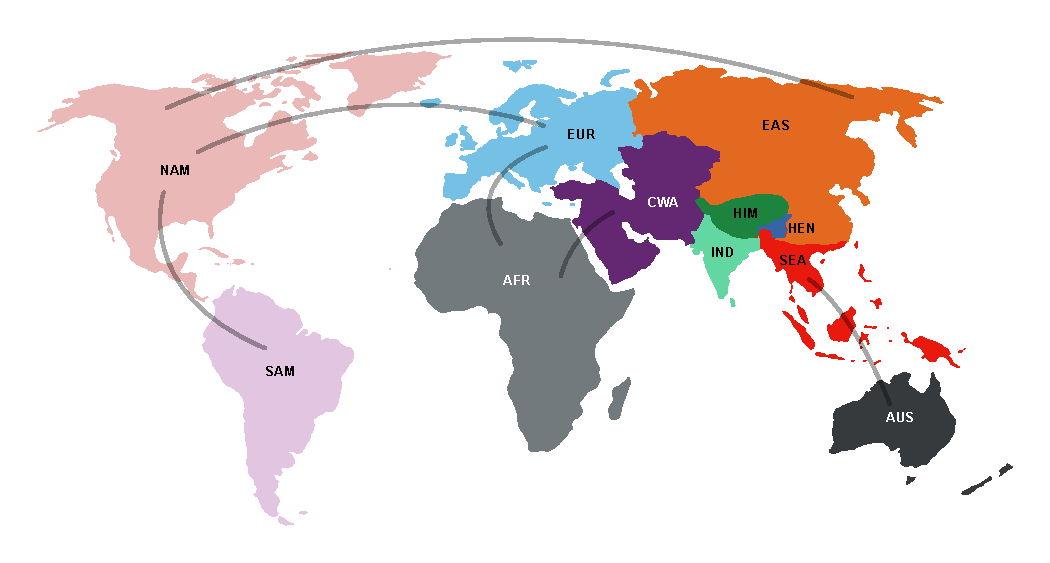
\includegraphics[width=.99\linewidth]{figures/regions.pdf}
\caption{Map of the 11 geographic regions used for ancestral range
  analyses in Lagrange.  HEN = Hengduan Mountains, HIM =
  Himalayas-QTP, EAS = temperate/boreal East Asia, SEA = Southeast
  Asia, CWA = Central/Western Asia, EUR = Europe, IND = India, AFR =
  Africa, NAM = North America, SAM = South America, AUS =
  Australasia. Lines and common borders indicate dispersal routes
  allowed in Lagrange.}
\label{fig:regions}
\end{figure}

\begin{figure}
  \caption{Reconstructions of ancestral geographic range (left) and
    net diversification rate (right) on the maximum clade credibility
    tree, with branch lengths set to posterior means, for each ingroup
    taxon (excluding \textit{Rhododendron}, shown as
    Fig.~5). Ancestral ranges are maximum-likelihood estimates at the
    start and end of each branch. Net diversification values are
    branch-segment means of the posterior distribution estimated by
    BAMM. Filled circles on the right indicate branches that appear in
    the 95\% credible set of distinct shift configurations, with the
    size and label of a circle indicating the cumulative probability
    of the branch over all configurations in the credible set. On the
    left, the marginal odds ratio for a shift in diversification
    regime along a branch is drawn for branches where the ratio
    exceeds 20. Geographic regions are coded as follows: HEN, Hengduan
    Mountains; HIM, Himalayas-QTP; EAS, temperate-boreal East Asia;
    SEA, Southeast Asia; CWA, central/western Asia; EUR, Europe; IND,
    India; AFR, Africa; NAM, North America; SAM, South America; AUS,
    Australasia.}
  \label{fig:ancranges}
\end{figure}

\addtocounter{figure}{-1}

\begin{figure}
\begin{subfigure}{\textwidth}
\centering
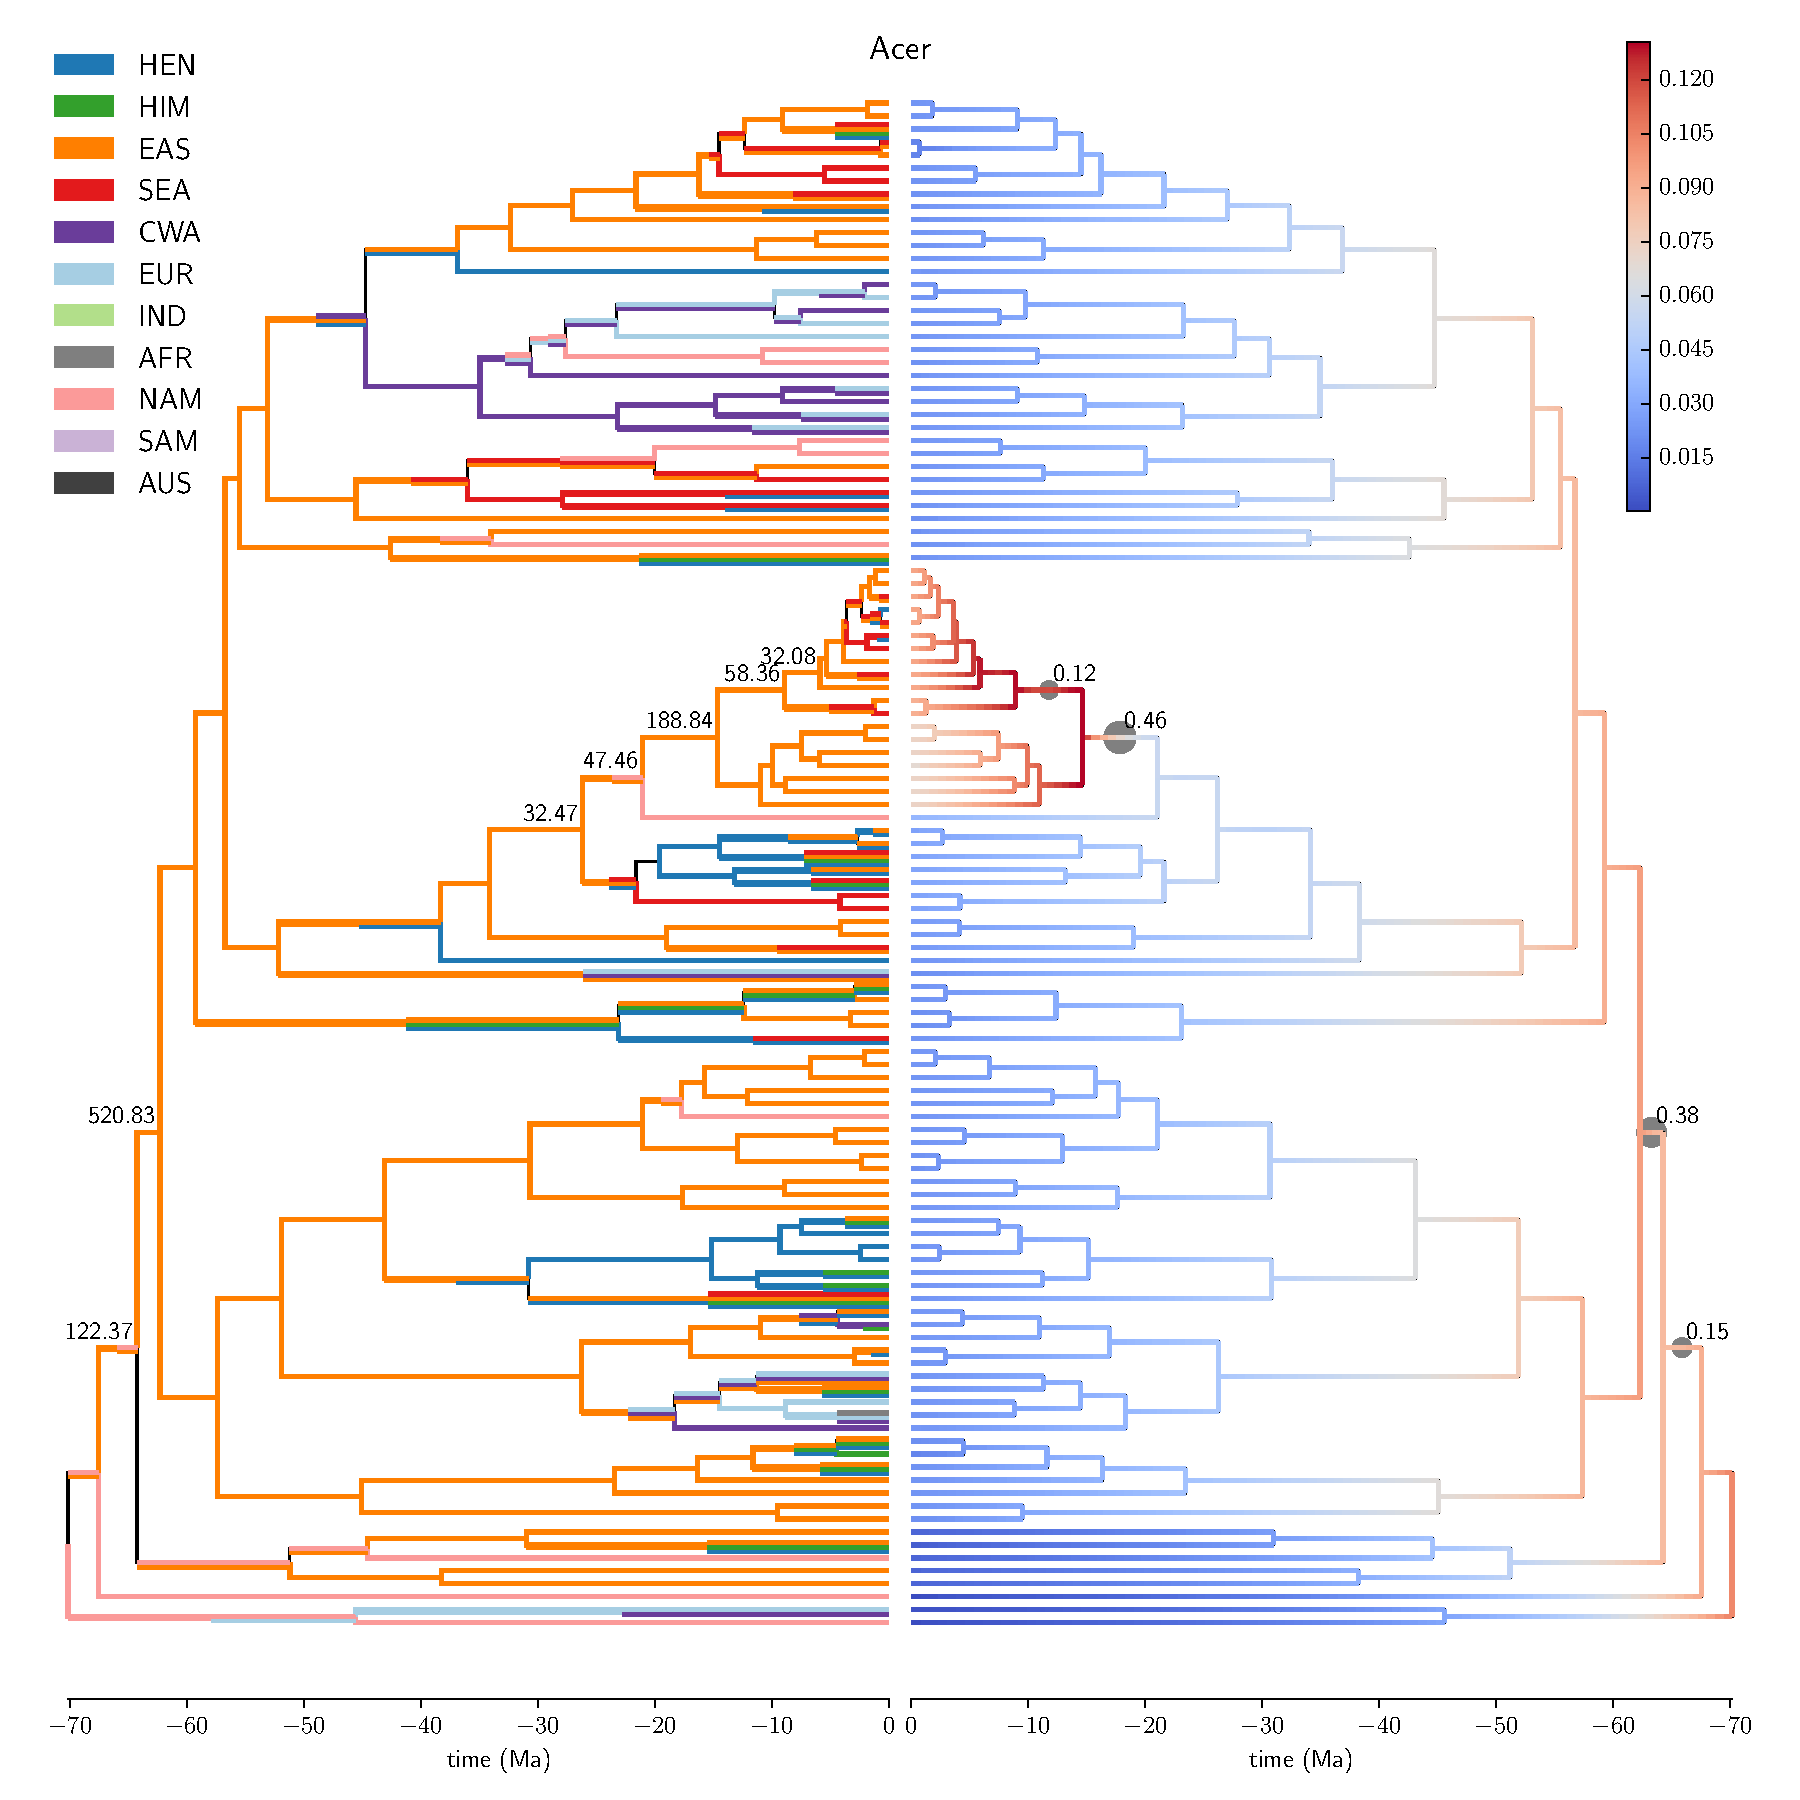
\includegraphics[width=.99\linewidth]{figures/Acer-supfig.pdf}
\label{fig:acer}
\caption{\textit{Acer}}
\end{subfigure}
\end{figure}

\begin{figure}
  \ContinuedFloat
\begin{subfigure}{\textwidth}
\centering
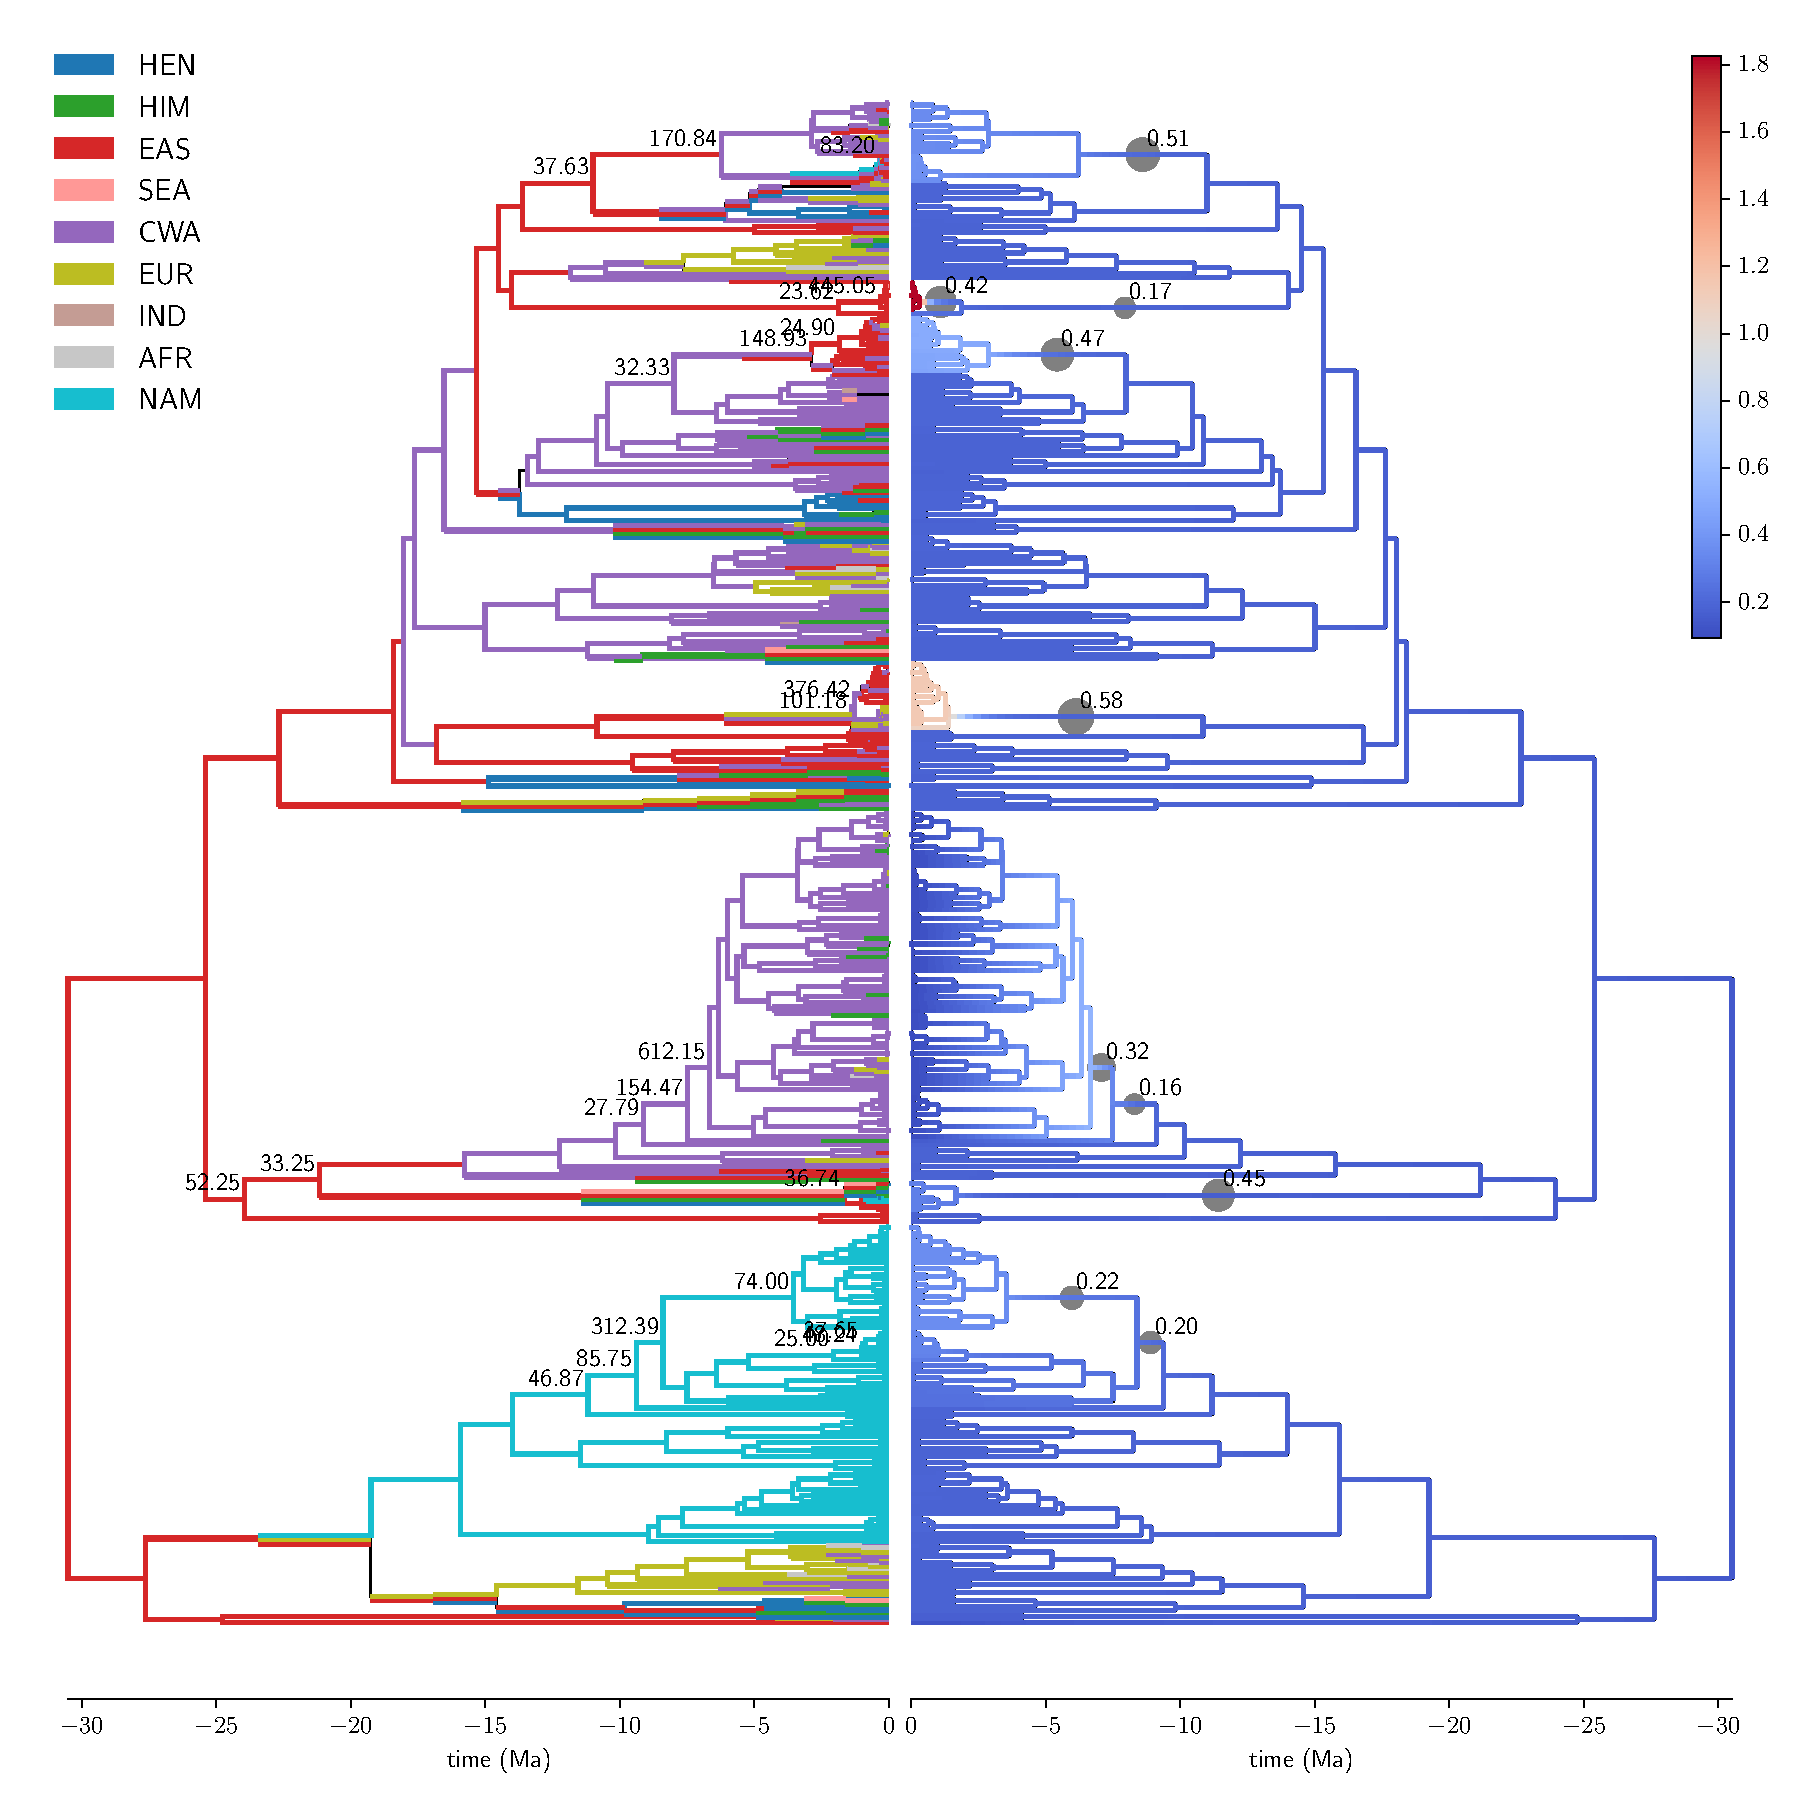
\includegraphics[width=.99\linewidth]{figures/Allium-supfig.pdf}
\label{fig:allium}
\caption{\textit{Allium}}
\end{subfigure}
\end{figure}

\begin{figure}
  \ContinuedFloat
\begin{subfigure}{\textwidth}
\centering
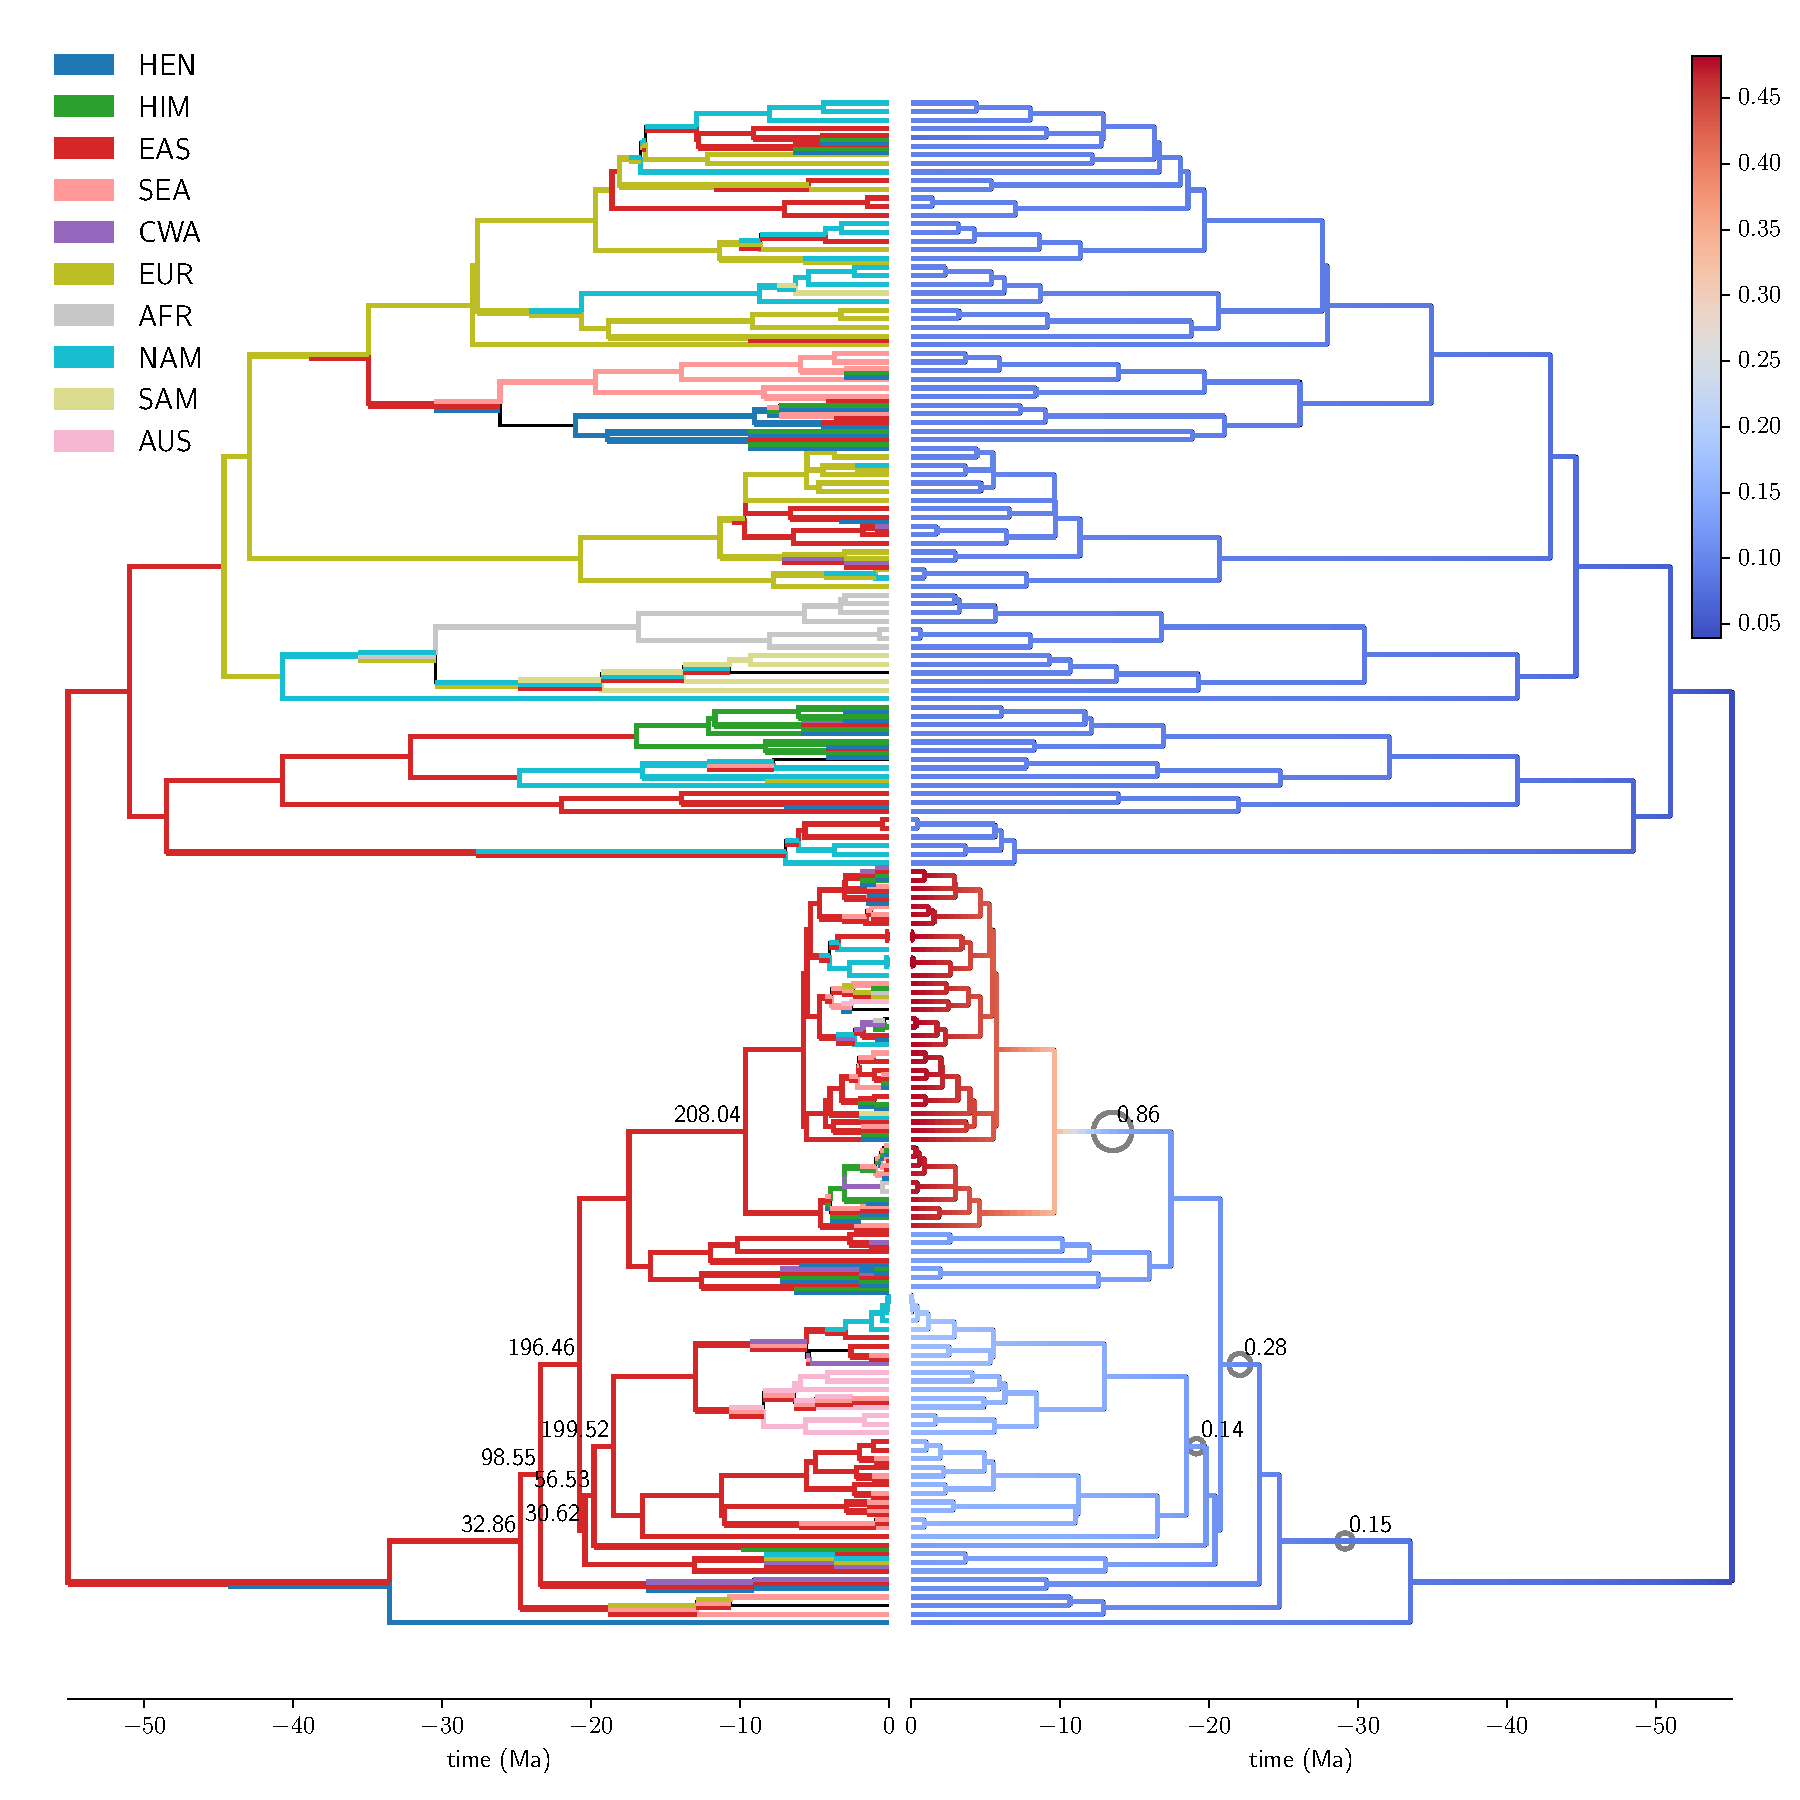
\includegraphics[width=.99\linewidth]{figures/Clematis-supfig.pdf}
\label{fig:allium}
\caption{Clematidinae+Anemoninae}
\end{subfigure}
\end{figure}

\begin{figure}
  \ContinuedFloat
\begin{subfigure}{\textwidth}
\centering
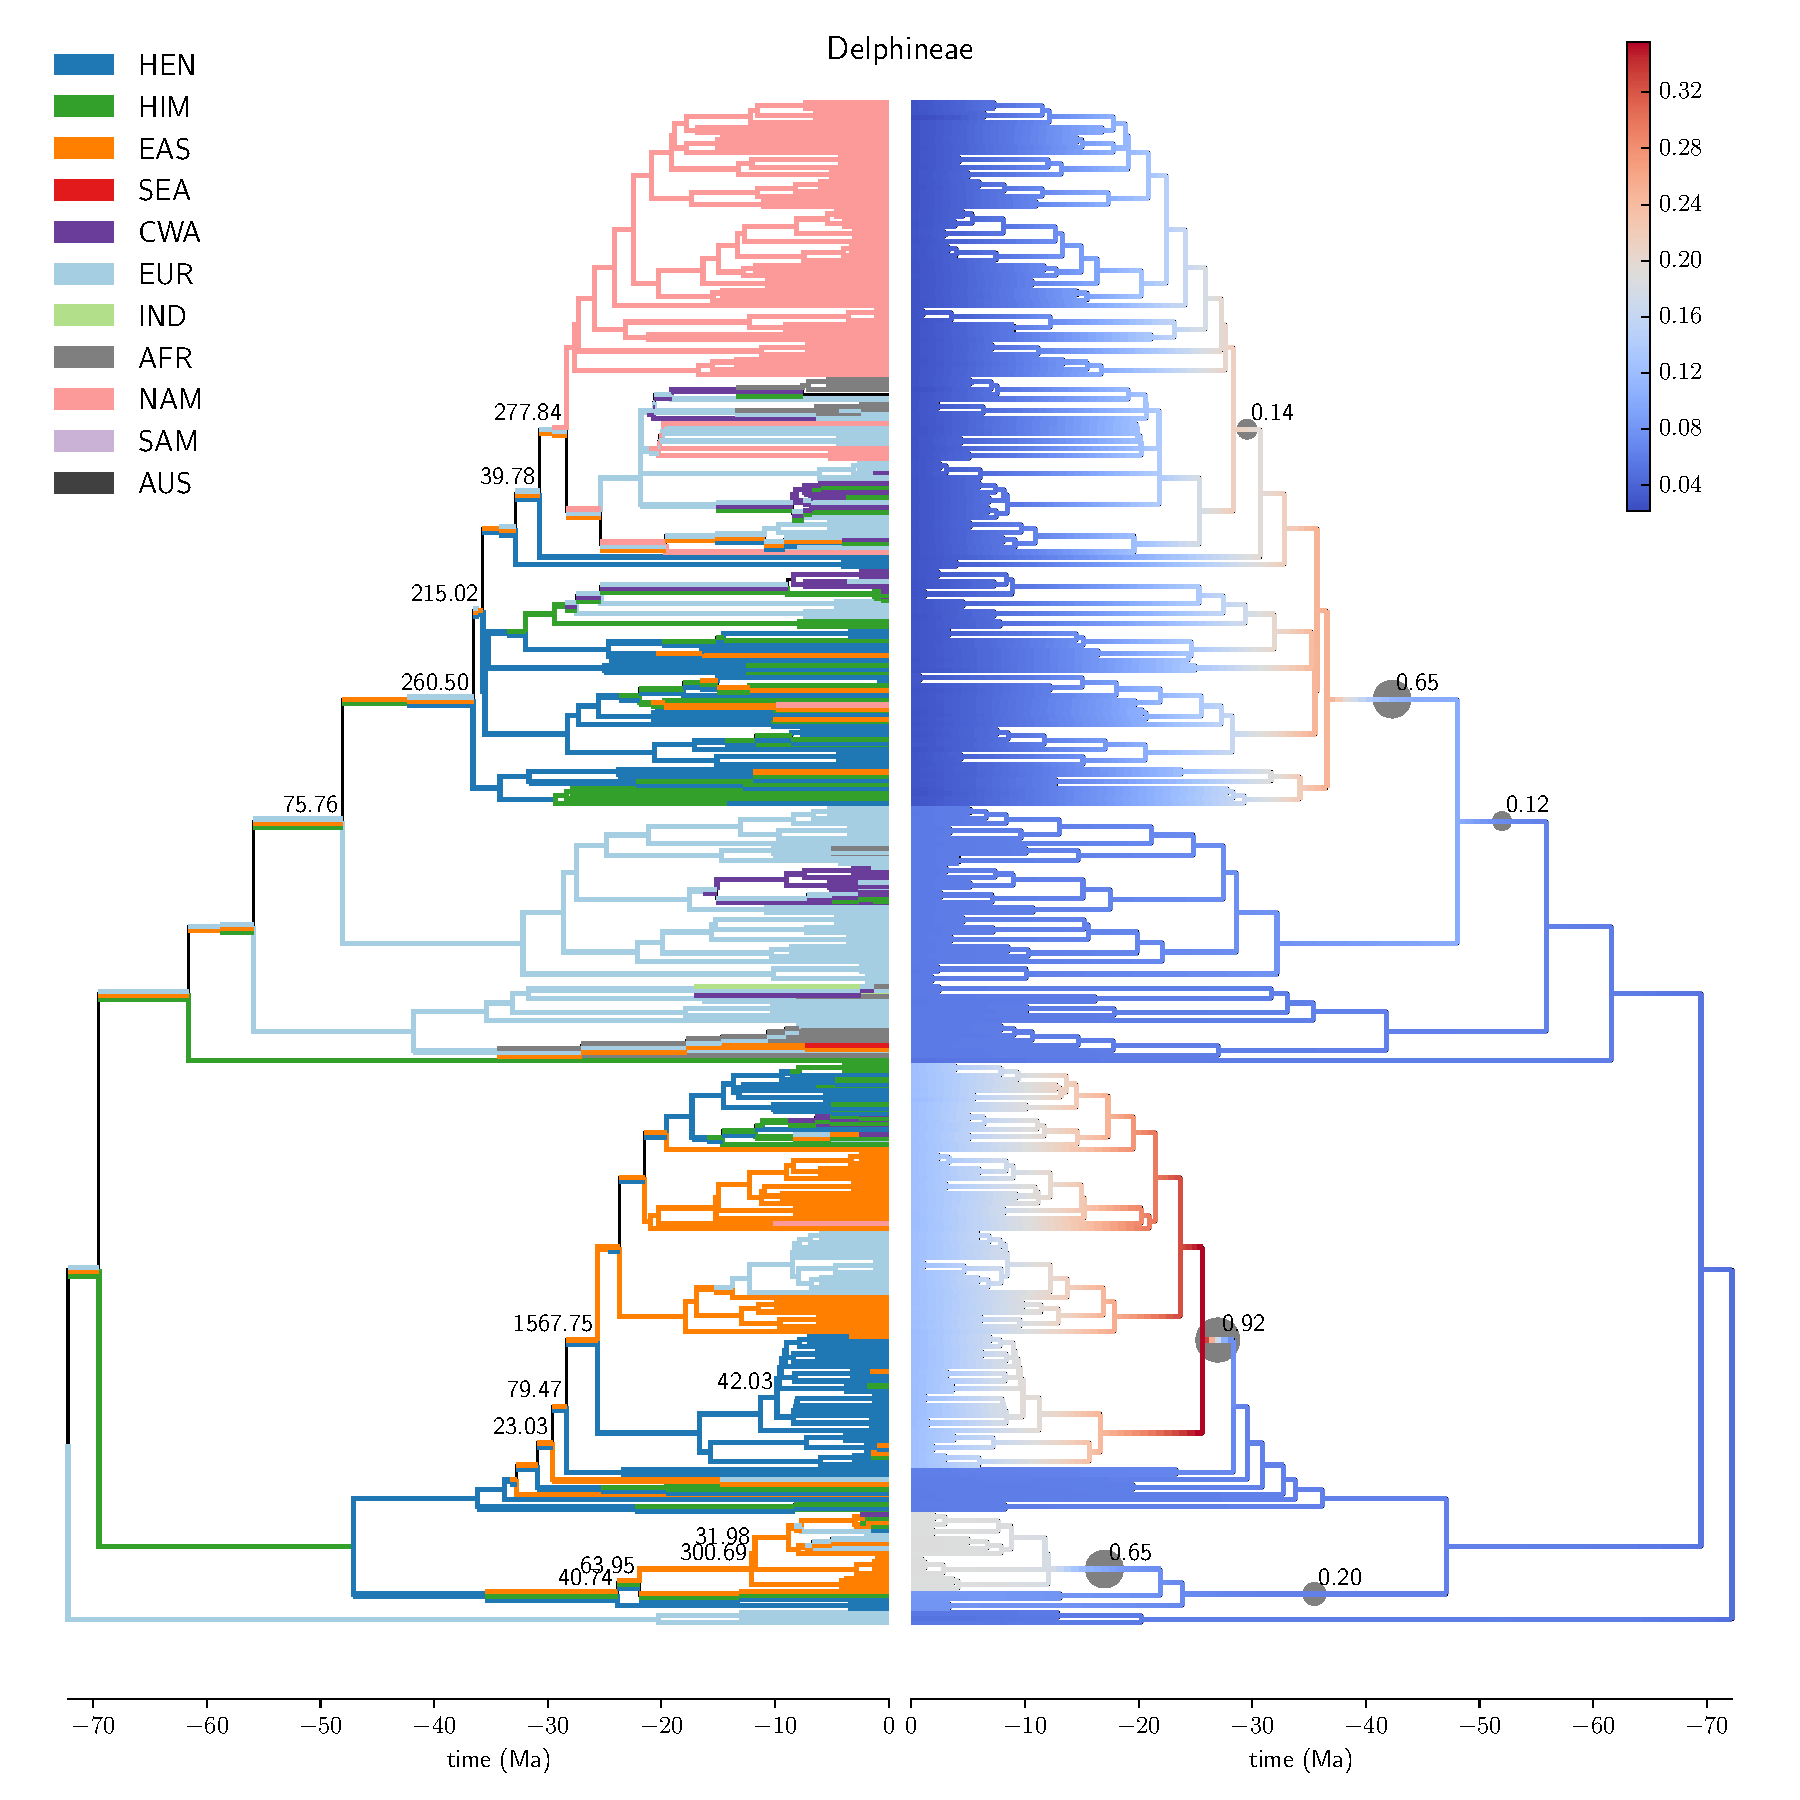
\includegraphics[width=.99\linewidth]{figures/Delphineae-supfig.pdf}
\label{fig:allium}
\caption{Delphineae}
\end{subfigure}
\end{figure}

\begin{figure}
  \ContinuedFloat
\begin{subfigure}{\textwidth}
\centering
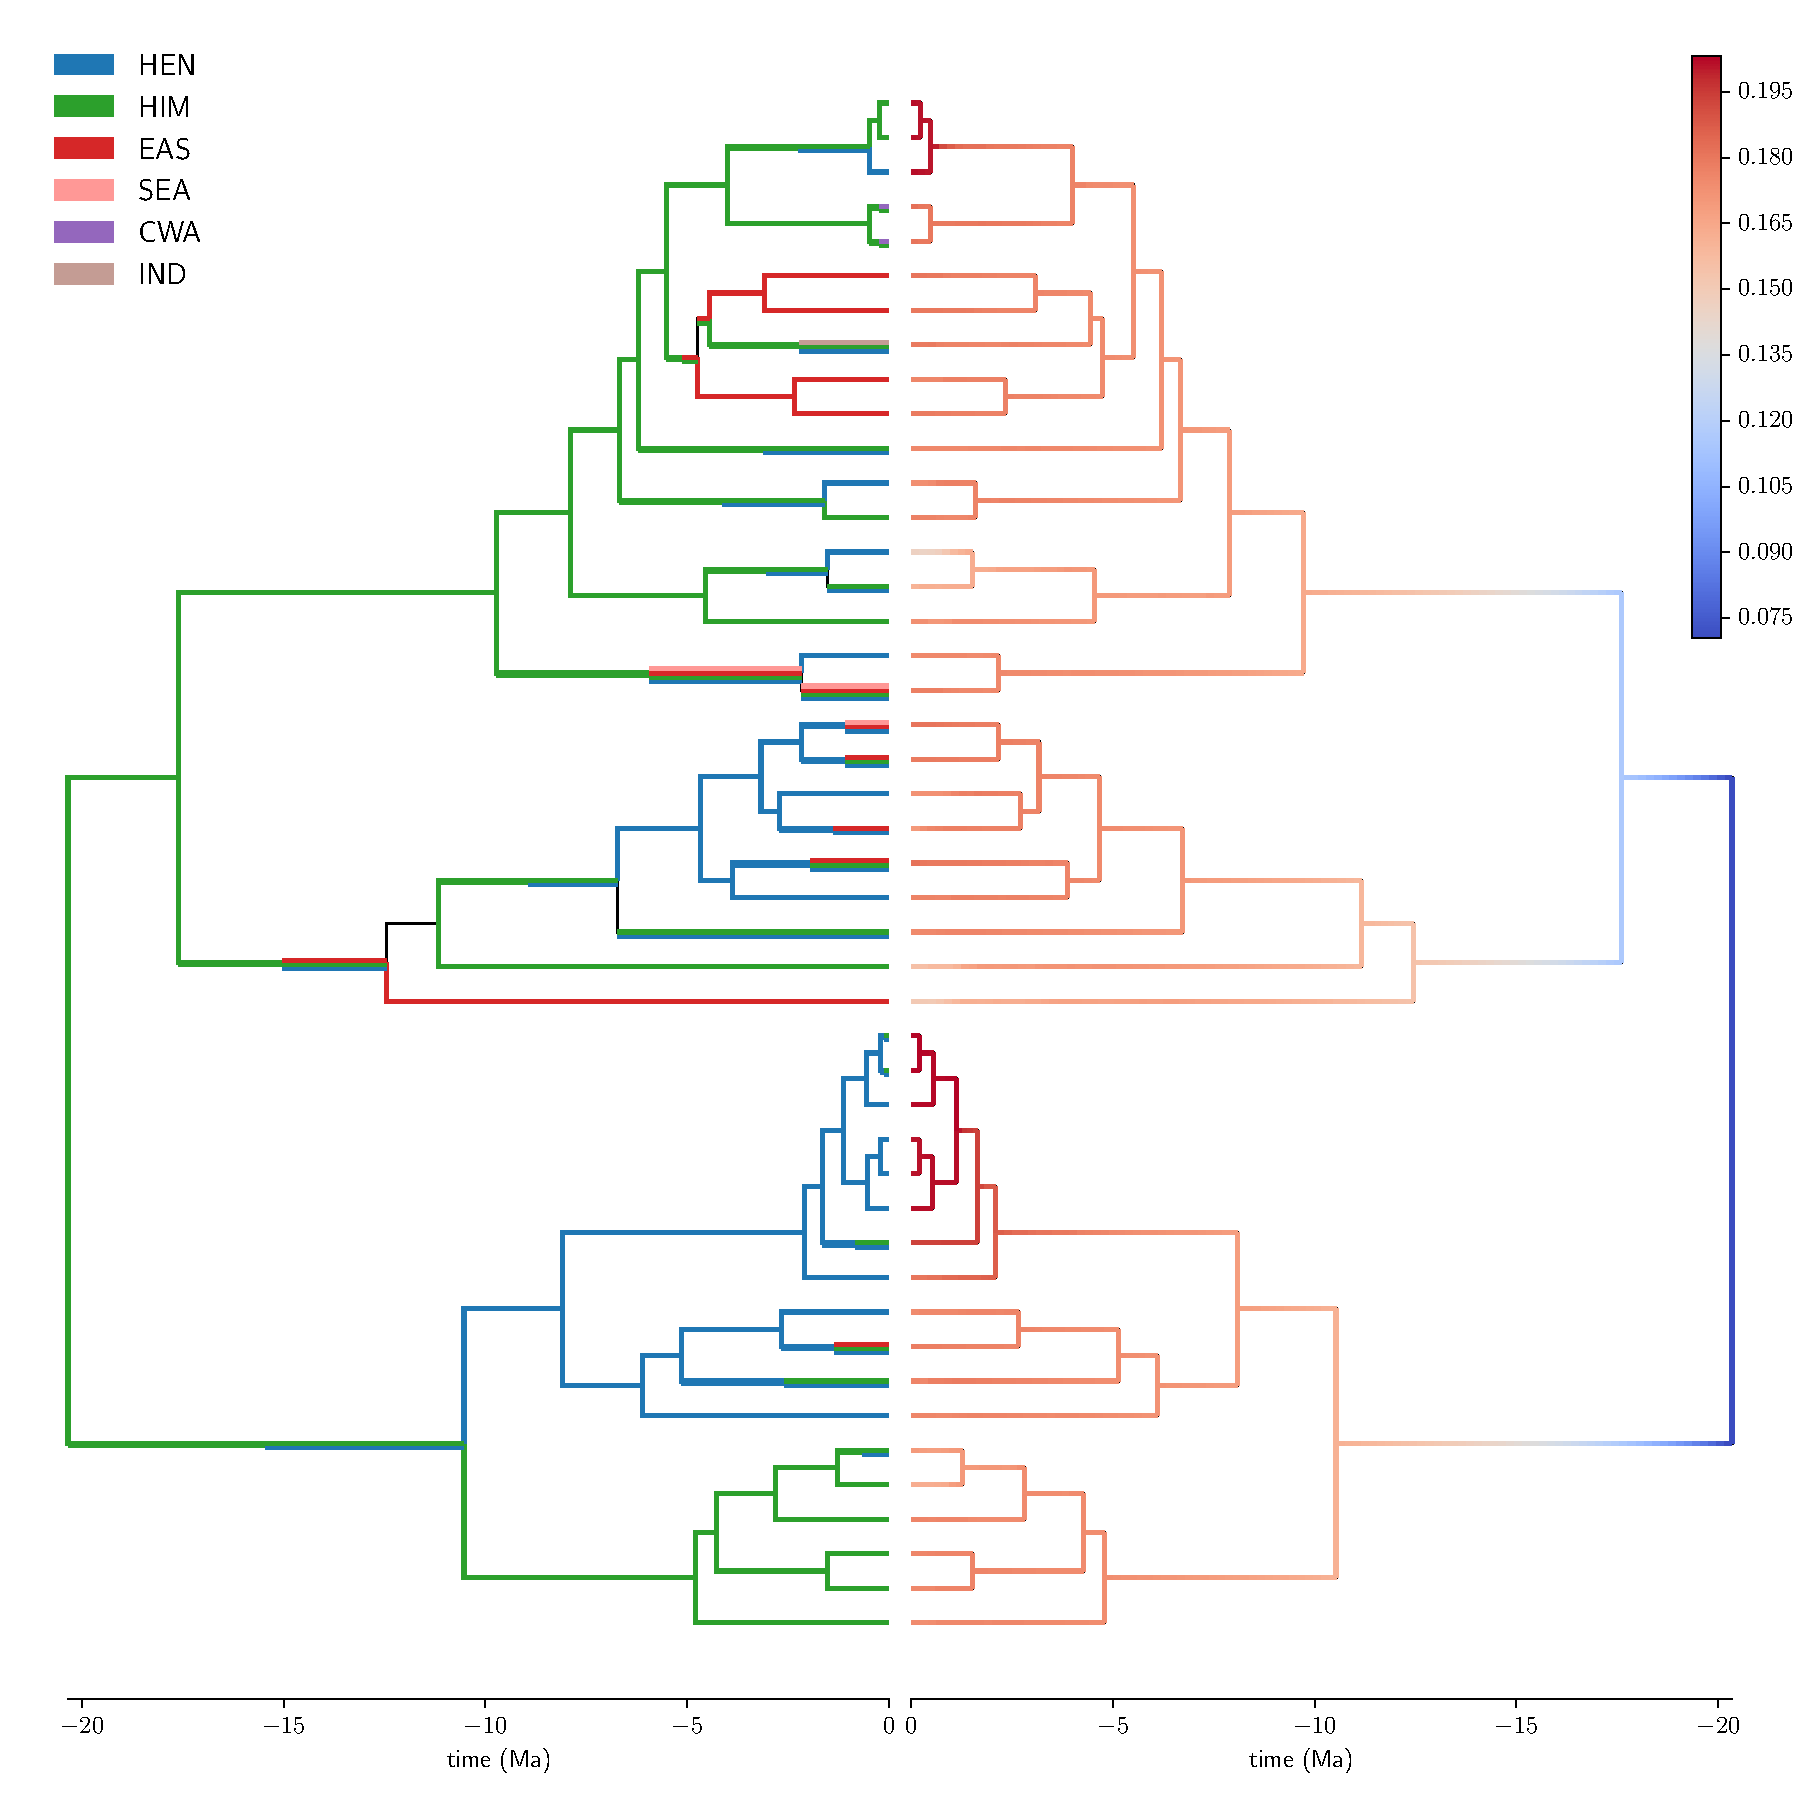
\includegraphics[width=.99\linewidth]{figures/Cyananthus-supfig.pdf}
\label{fig:allium}
\caption{\textit{Cyananthus}}
\end{subfigure}
\end{figure}

\begin{figure}
  \ContinuedFloat
\begin{subfigure}{\textwidth}
\centering
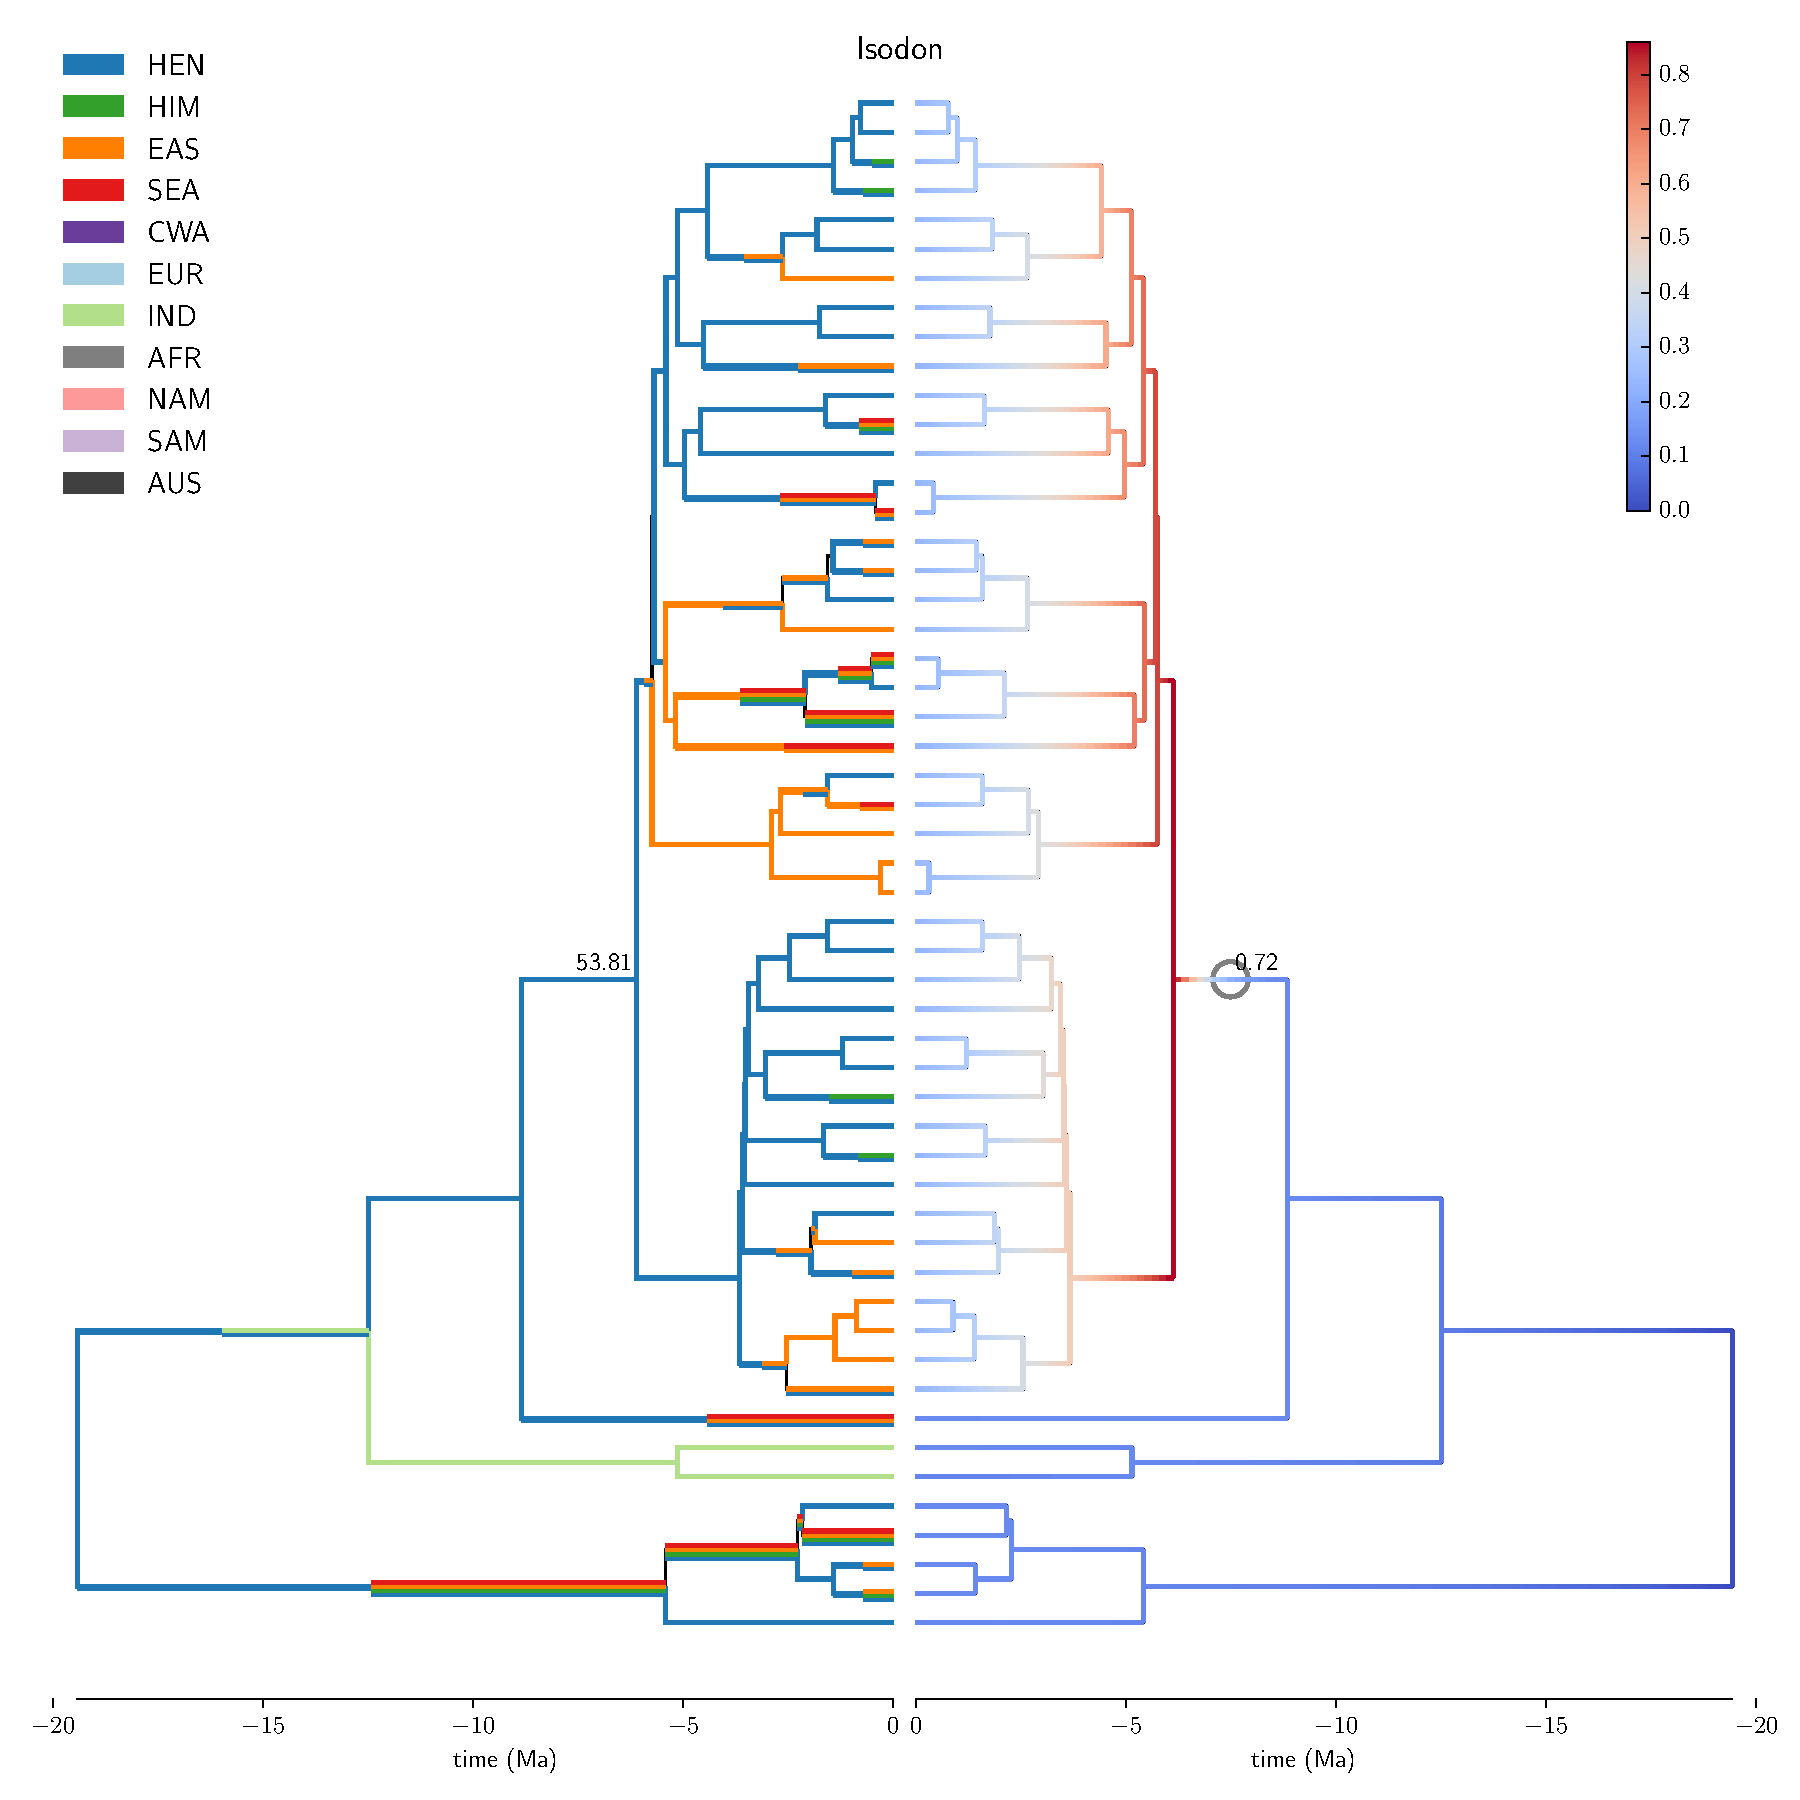
\includegraphics[width=.99\linewidth]{figures/Isodon-supfig.pdf}
\label{fig:allium}
\caption{\textit{Isodon}}
\end{subfigure}
\end{figure}

\begin{figure}
  \ContinuedFloat
\begin{subfigure}{\textwidth}
\centering
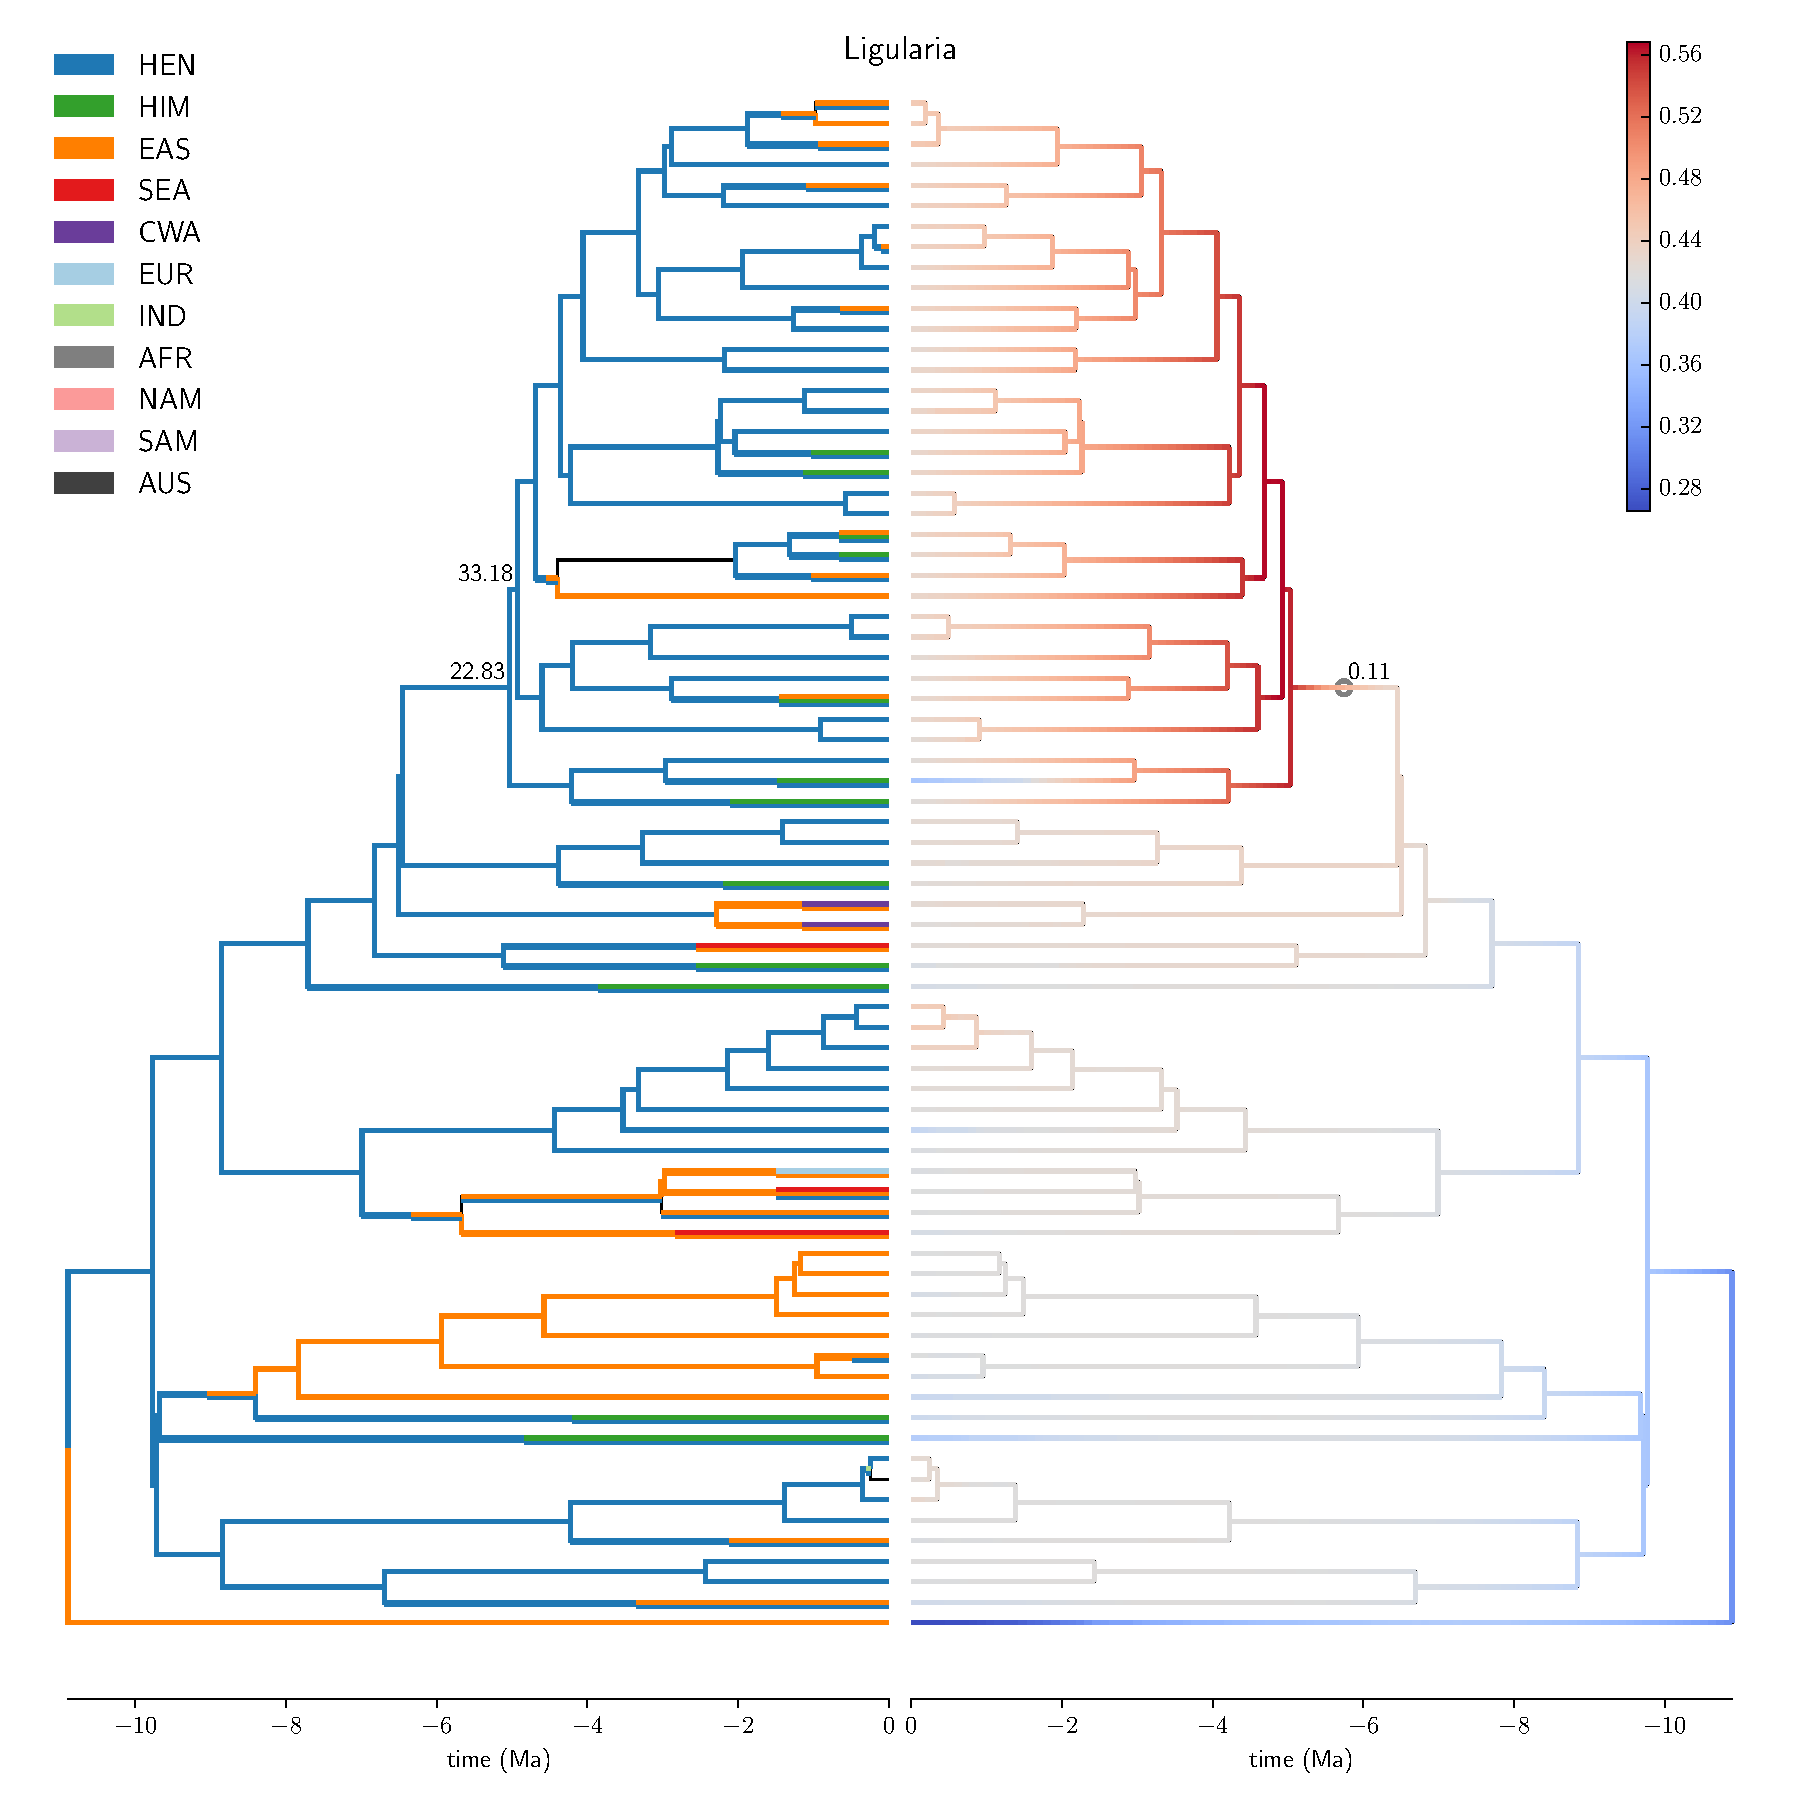
\includegraphics[width=.99\linewidth]{figures/Ligularia-supfig.pdf}
\label{fig:allium}
\caption{\textit{Ligularia-Cremanthodium-Parasenecio} complex}
\end{subfigure}
\end{figure}

\begin{figure}
  \ContinuedFloat
\begin{subfigure}{\textwidth}
\centering
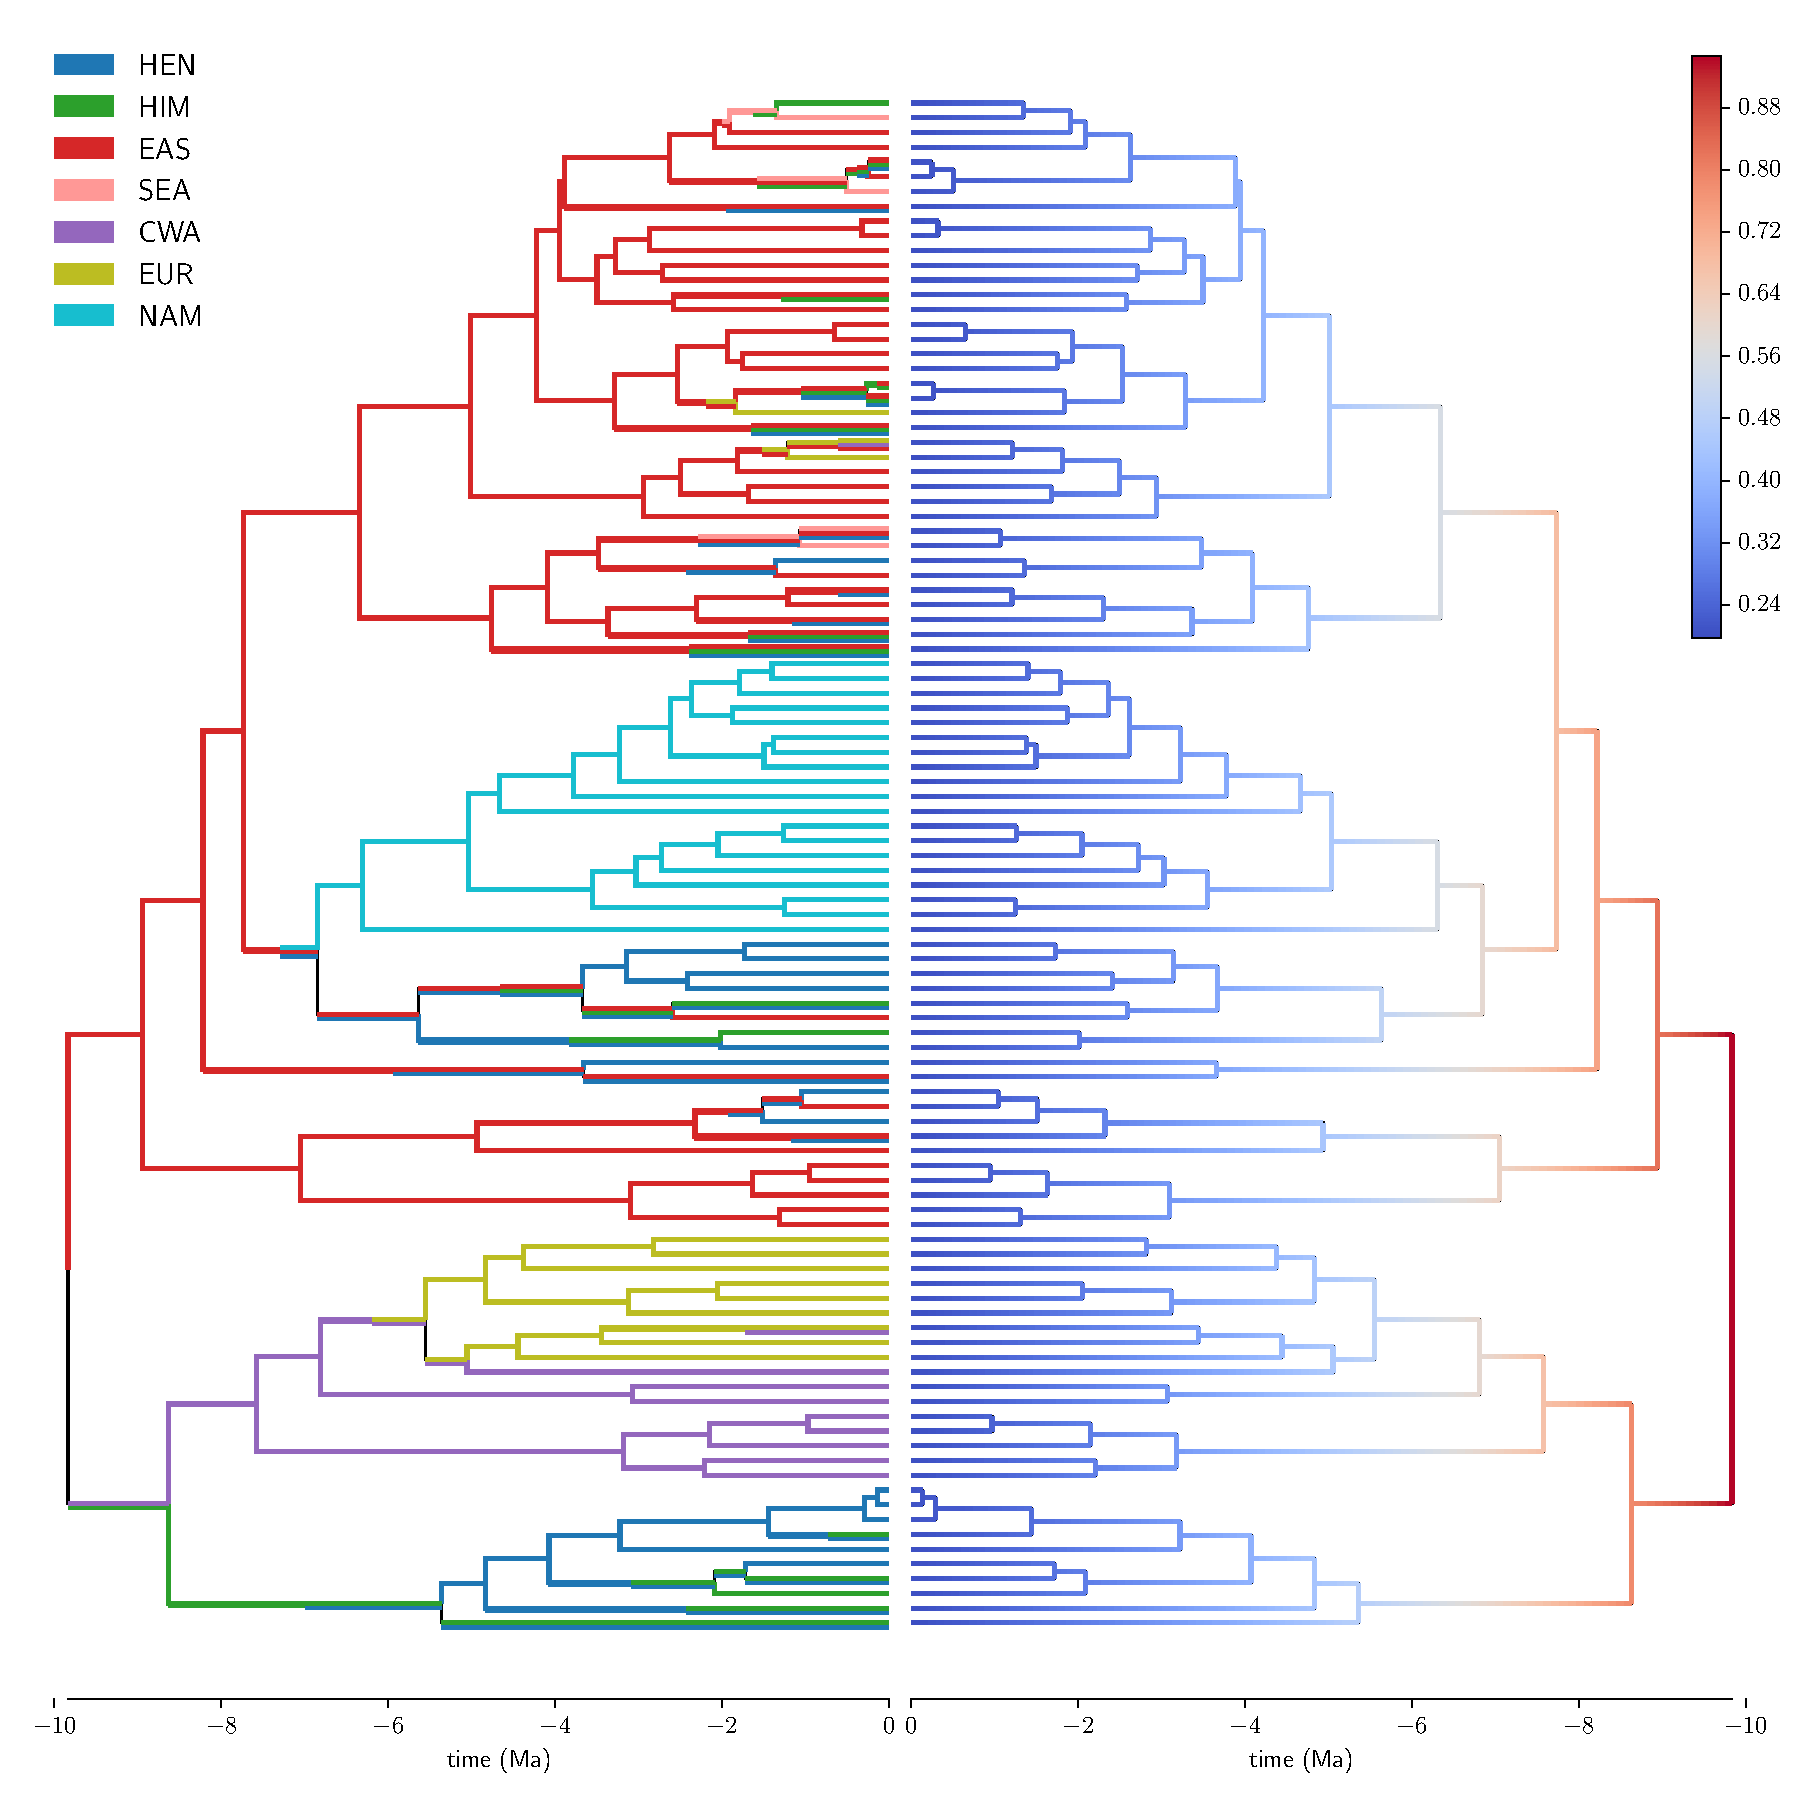
\includegraphics[width=.99\linewidth]{figures/Lilium-supfig.pdf}
\label{fig:allium}
\caption{\textit{Lilium} (including \textit{Nomocharis})}
\end{subfigure}
\end{figure}

\begin{figure}
  \ContinuedFloat
\begin{subfigure}{\textwidth}
\centering
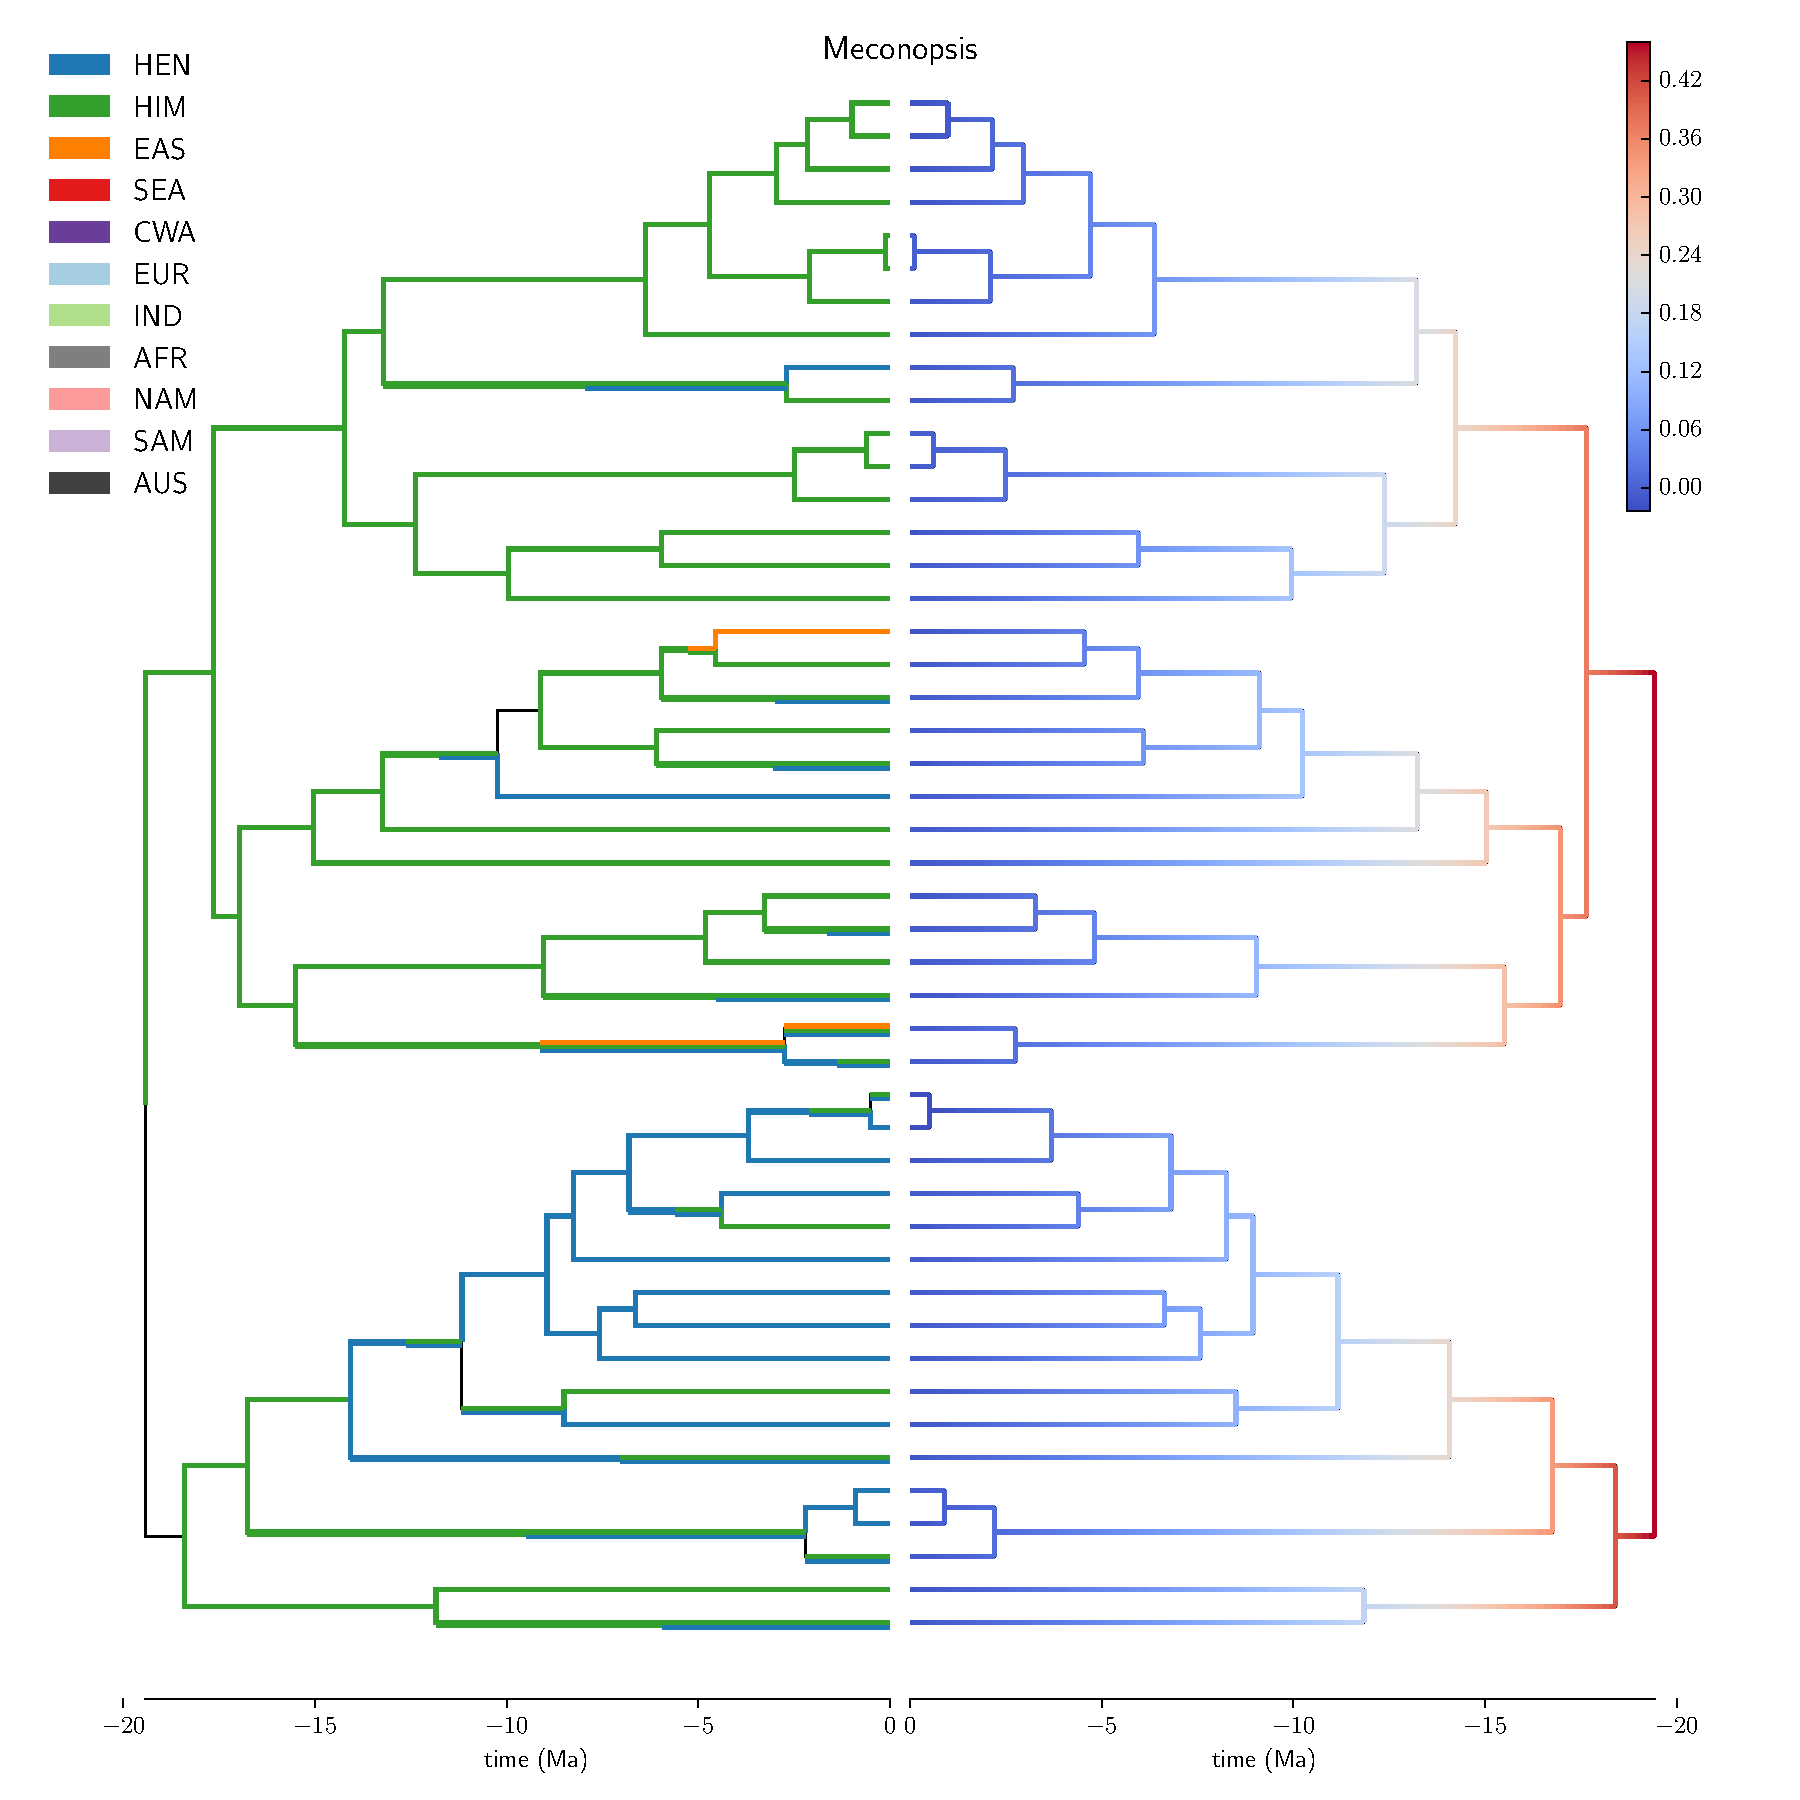
\includegraphics[width=.99\linewidth]{figures/Meconopsis-supfig.pdf}
\label{fig:allium}
\caption{\textit{Meconopsis}}
\end{subfigure}
\end{figure}

\begin{figure}
  \ContinuedFloat
\begin{subfigure}{\textwidth}
\centering
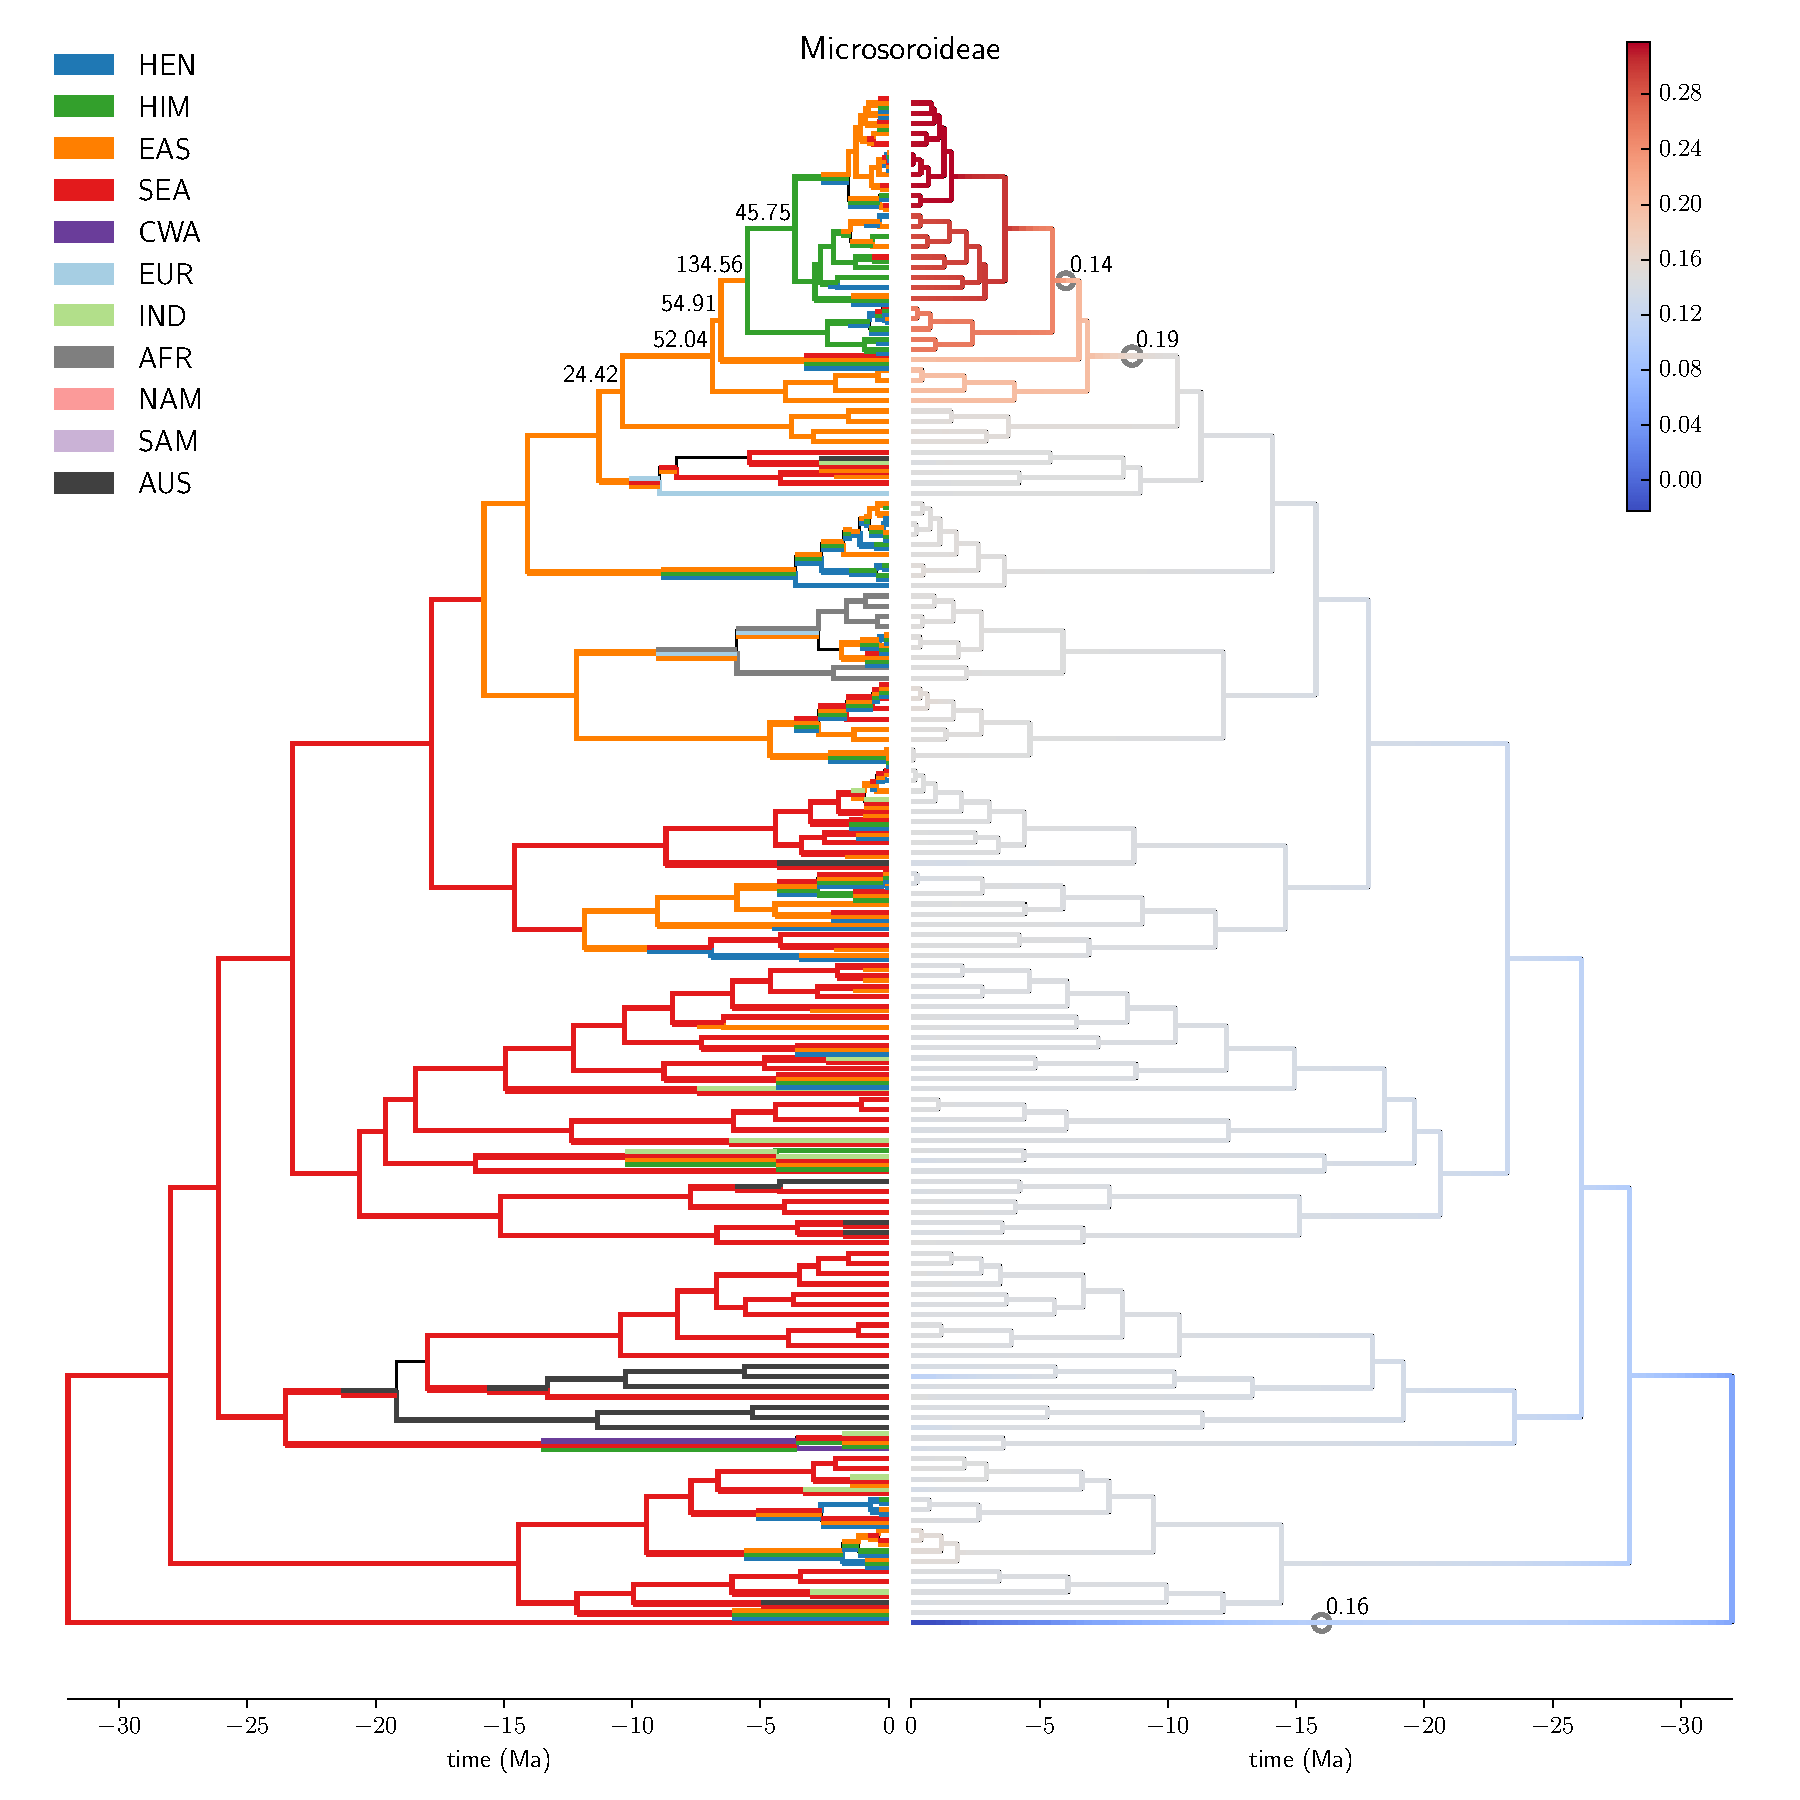
\includegraphics[width=.99\linewidth]{figures/Microsoroideae-supfig.pdf}
\label{fig:allium}
\caption{Microsoroideae}
\end{subfigure}
\end{figure}

\begin{figure}
  \ContinuedFloat
\begin{subfigure}{\textwidth}
\centering
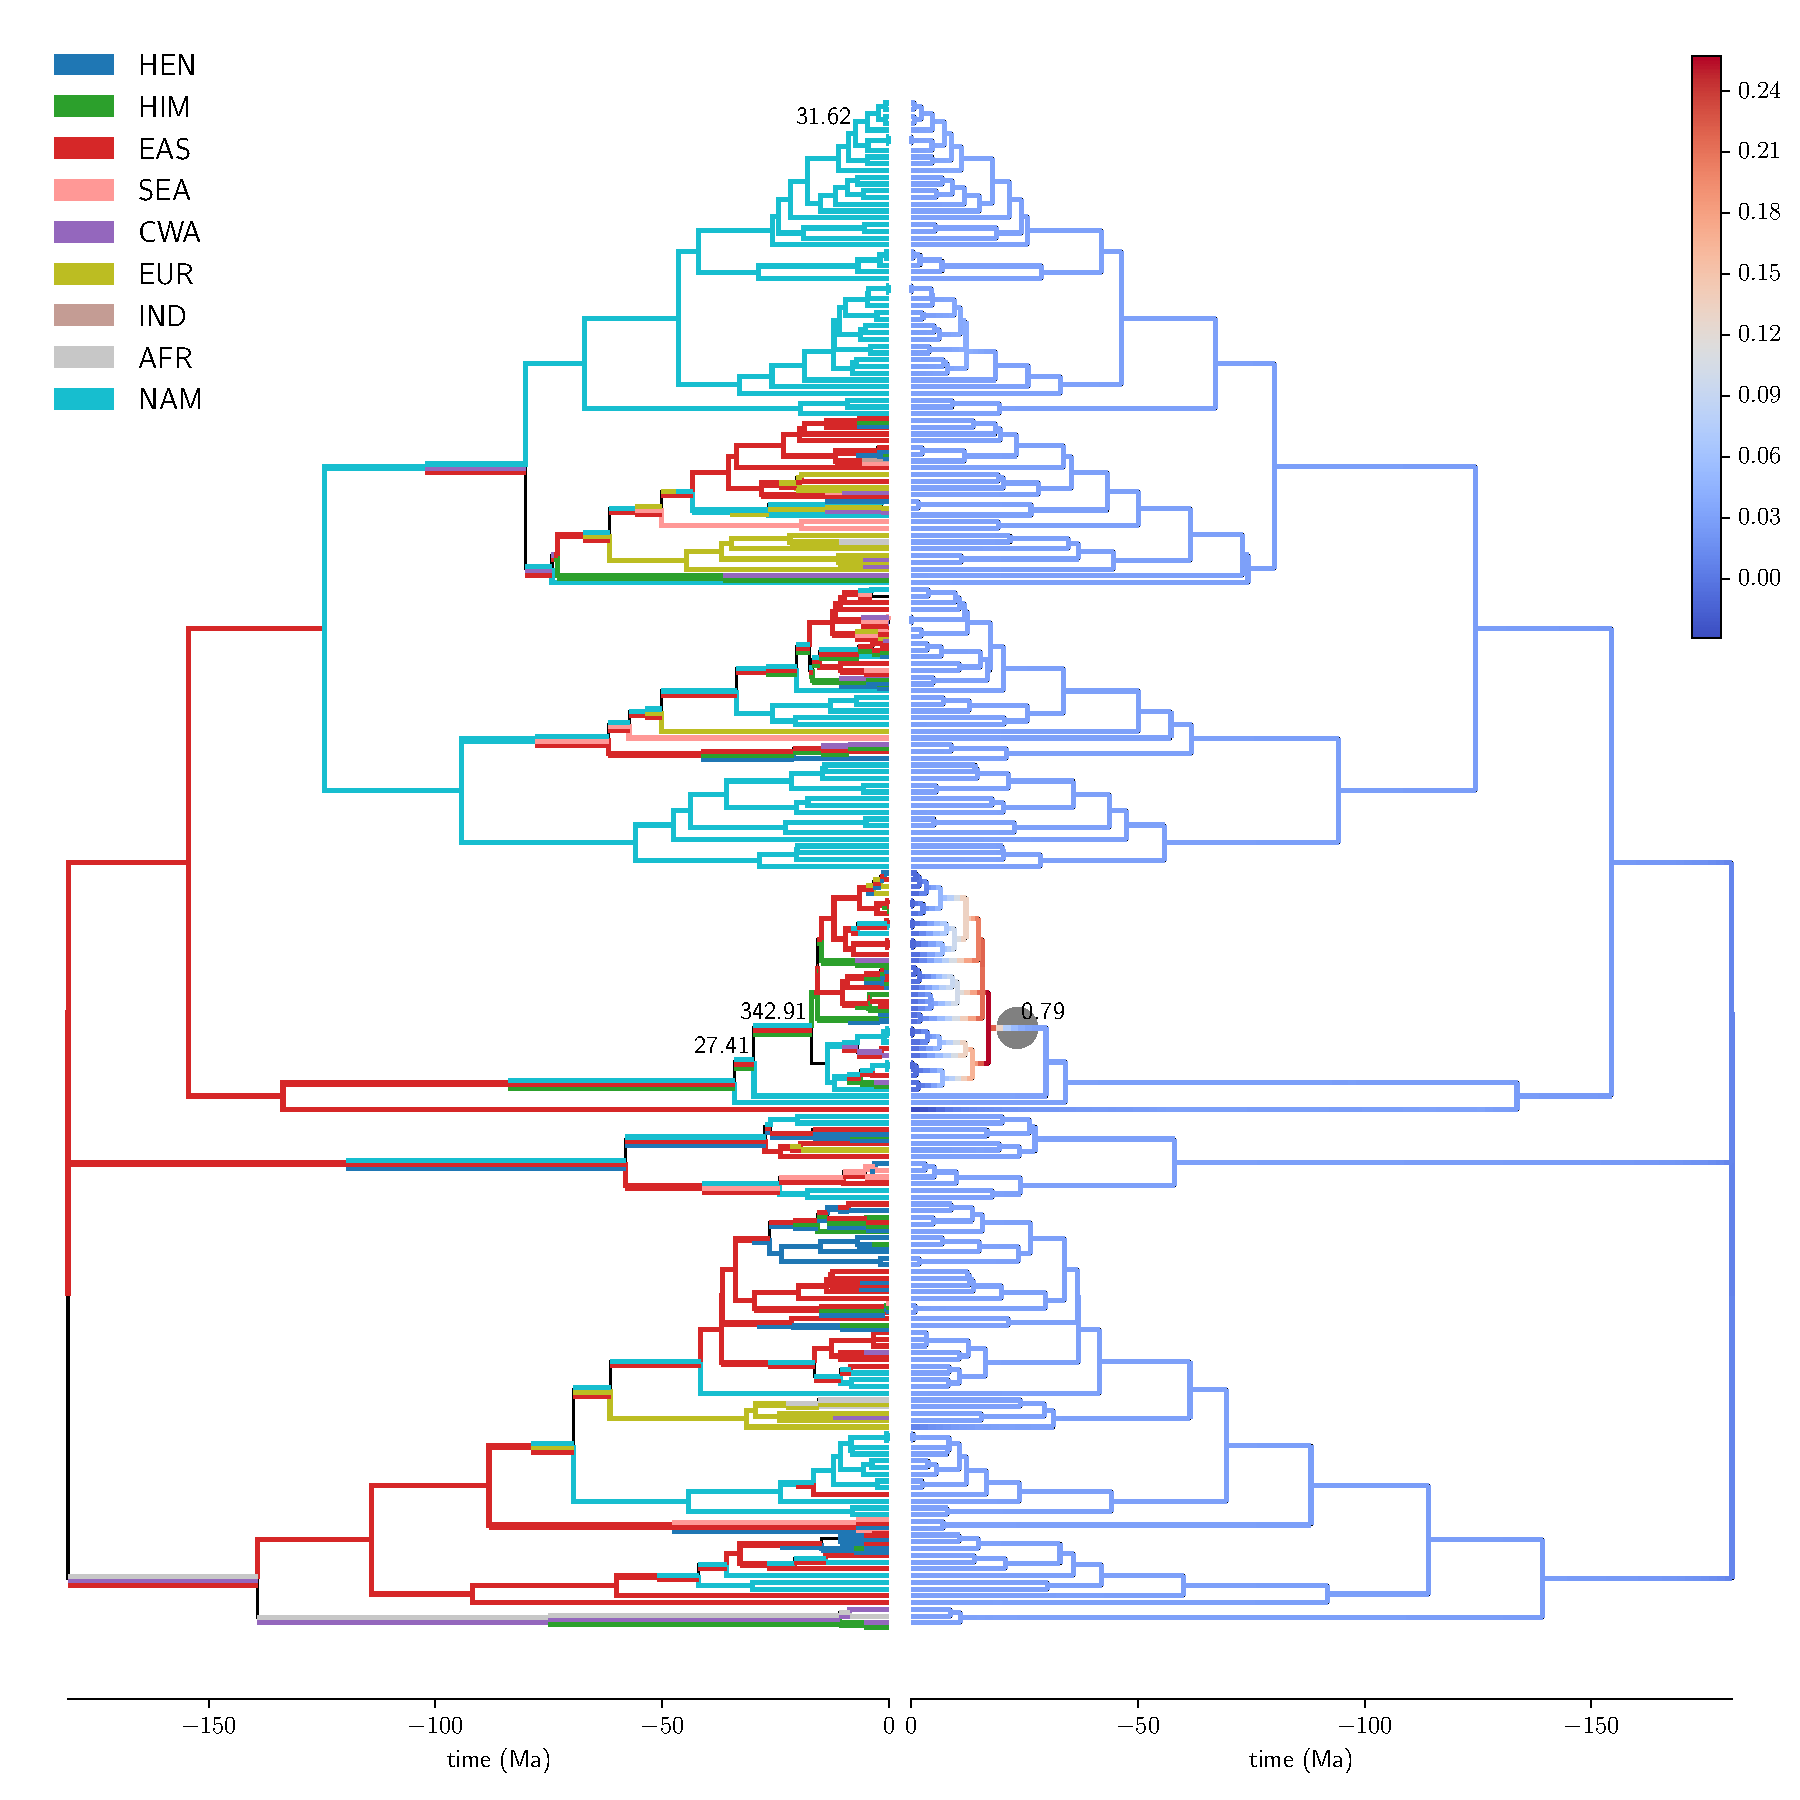
\includegraphics[width=.99\linewidth]{figures/Pinaceae-supfig.pdf}
\label{fig:allium}
\caption{Pinaceae}
\end{subfigure}
\end{figure}

\begin{figure}
  \ContinuedFloat
\begin{subfigure}{\textwidth}
\centering
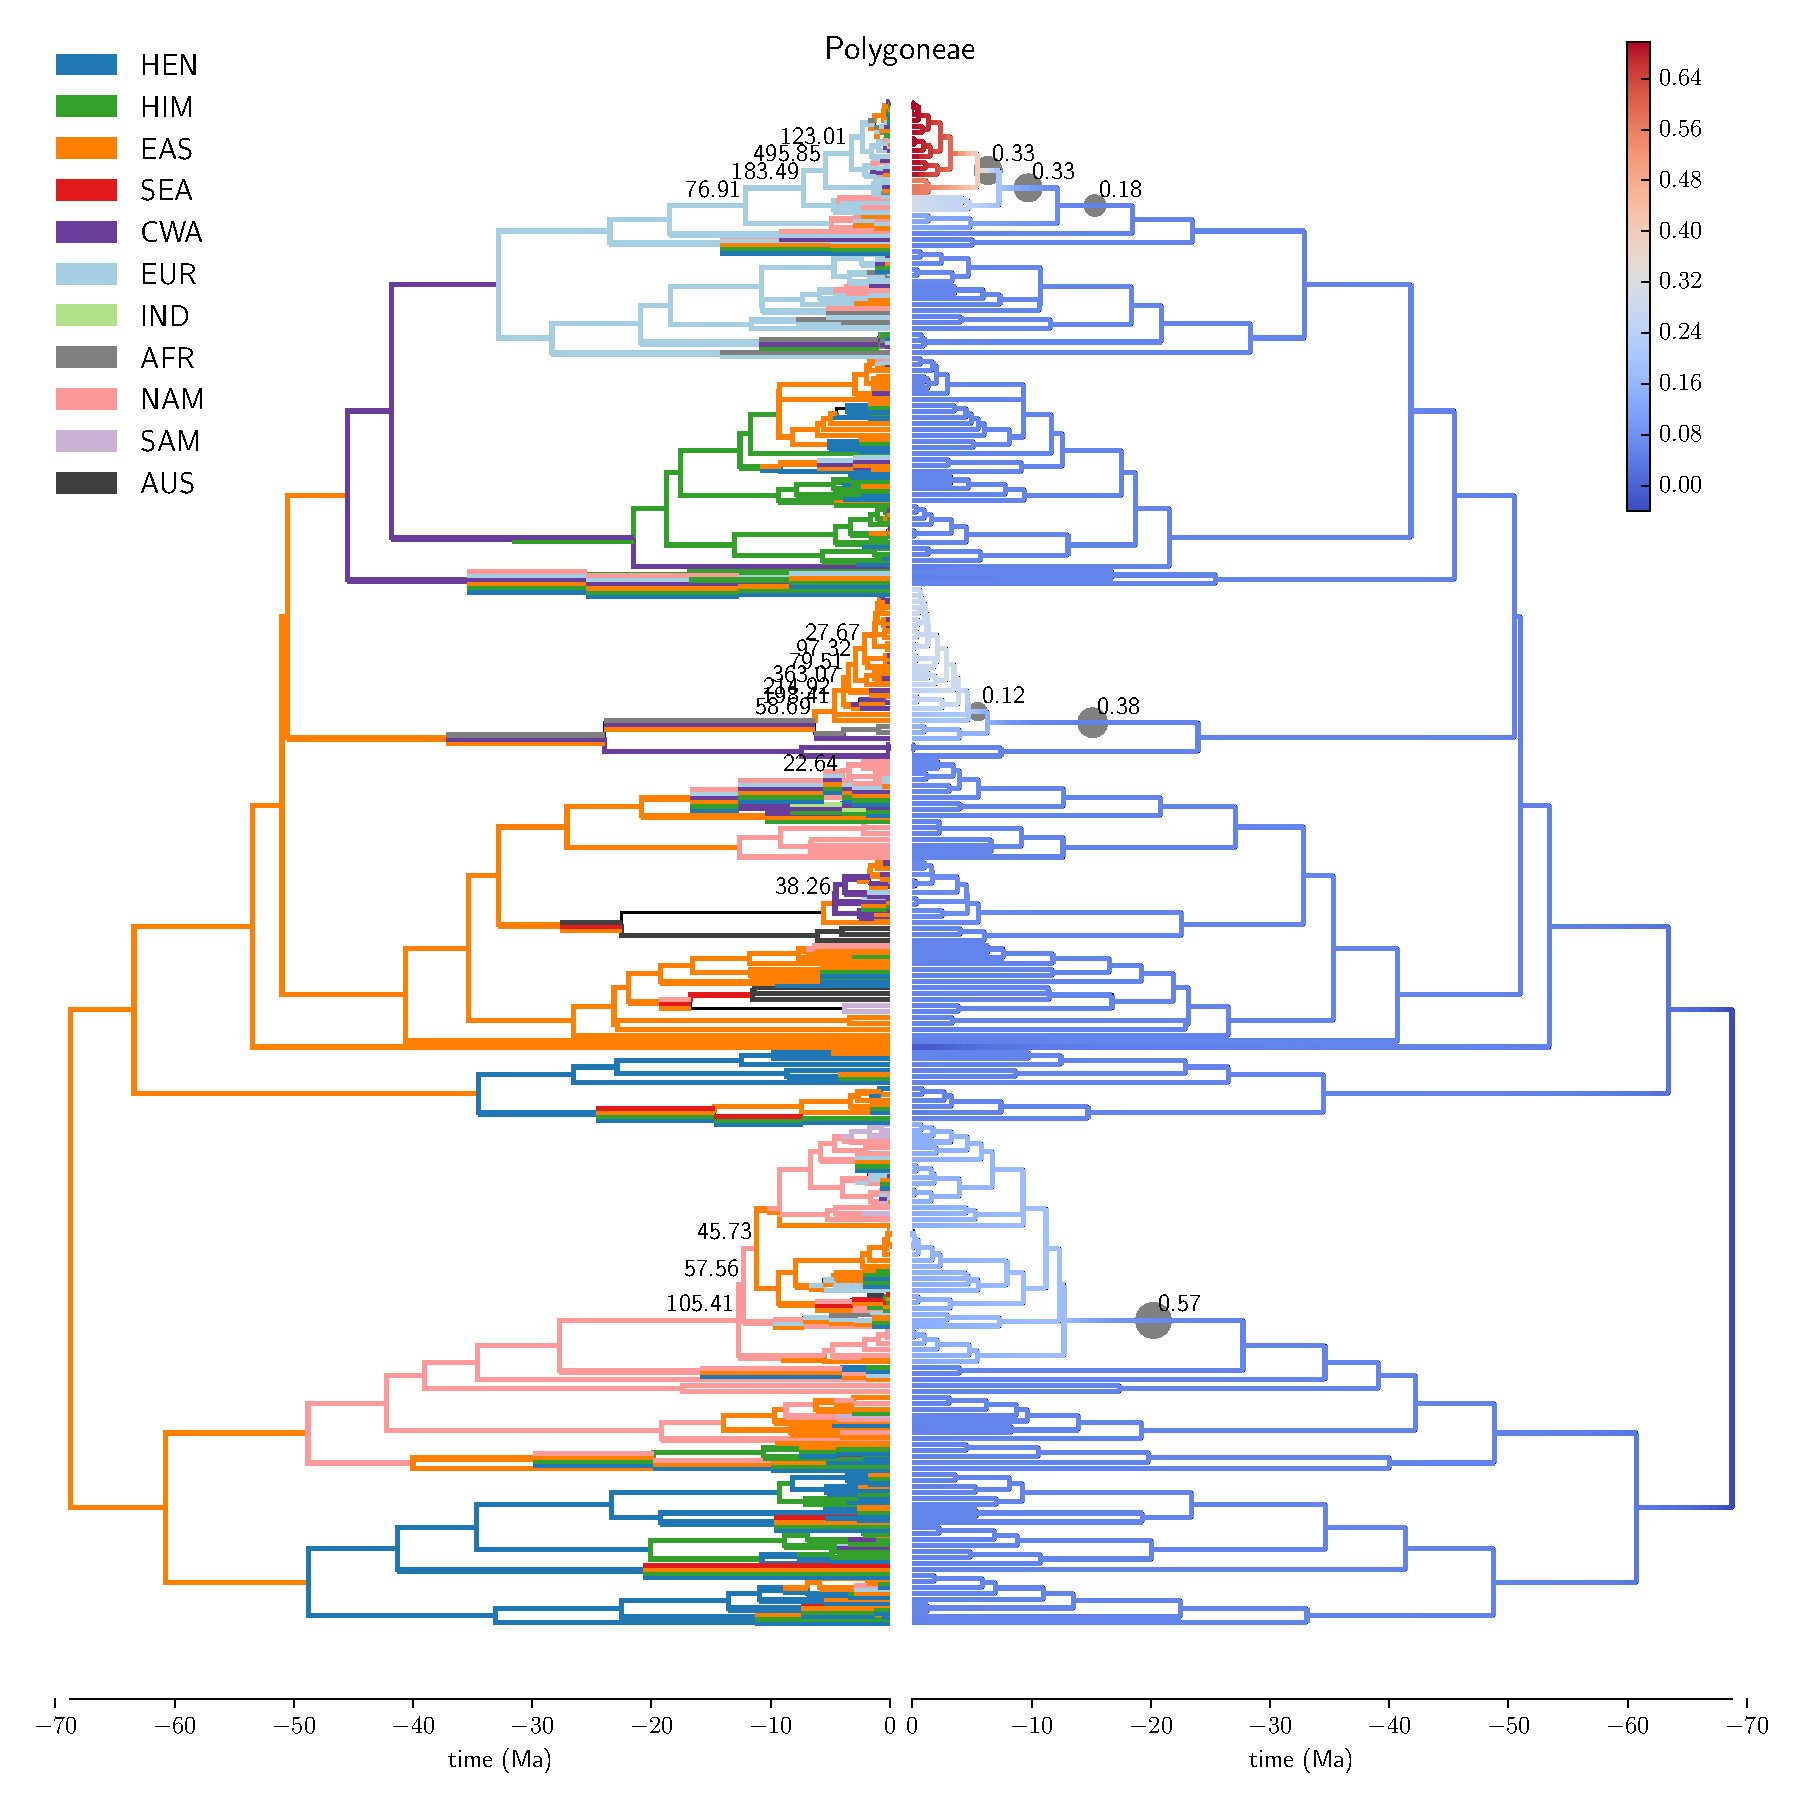
\includegraphics[width=.99\linewidth]{figures/Polygoneae-supfig.pdf}
\label{fig:allium}
\caption{Polygoneae}
\end{subfigure}
\end{figure}

\begin{figure}
  \ContinuedFloat
\begin{subfigure}{\textwidth}
\centering
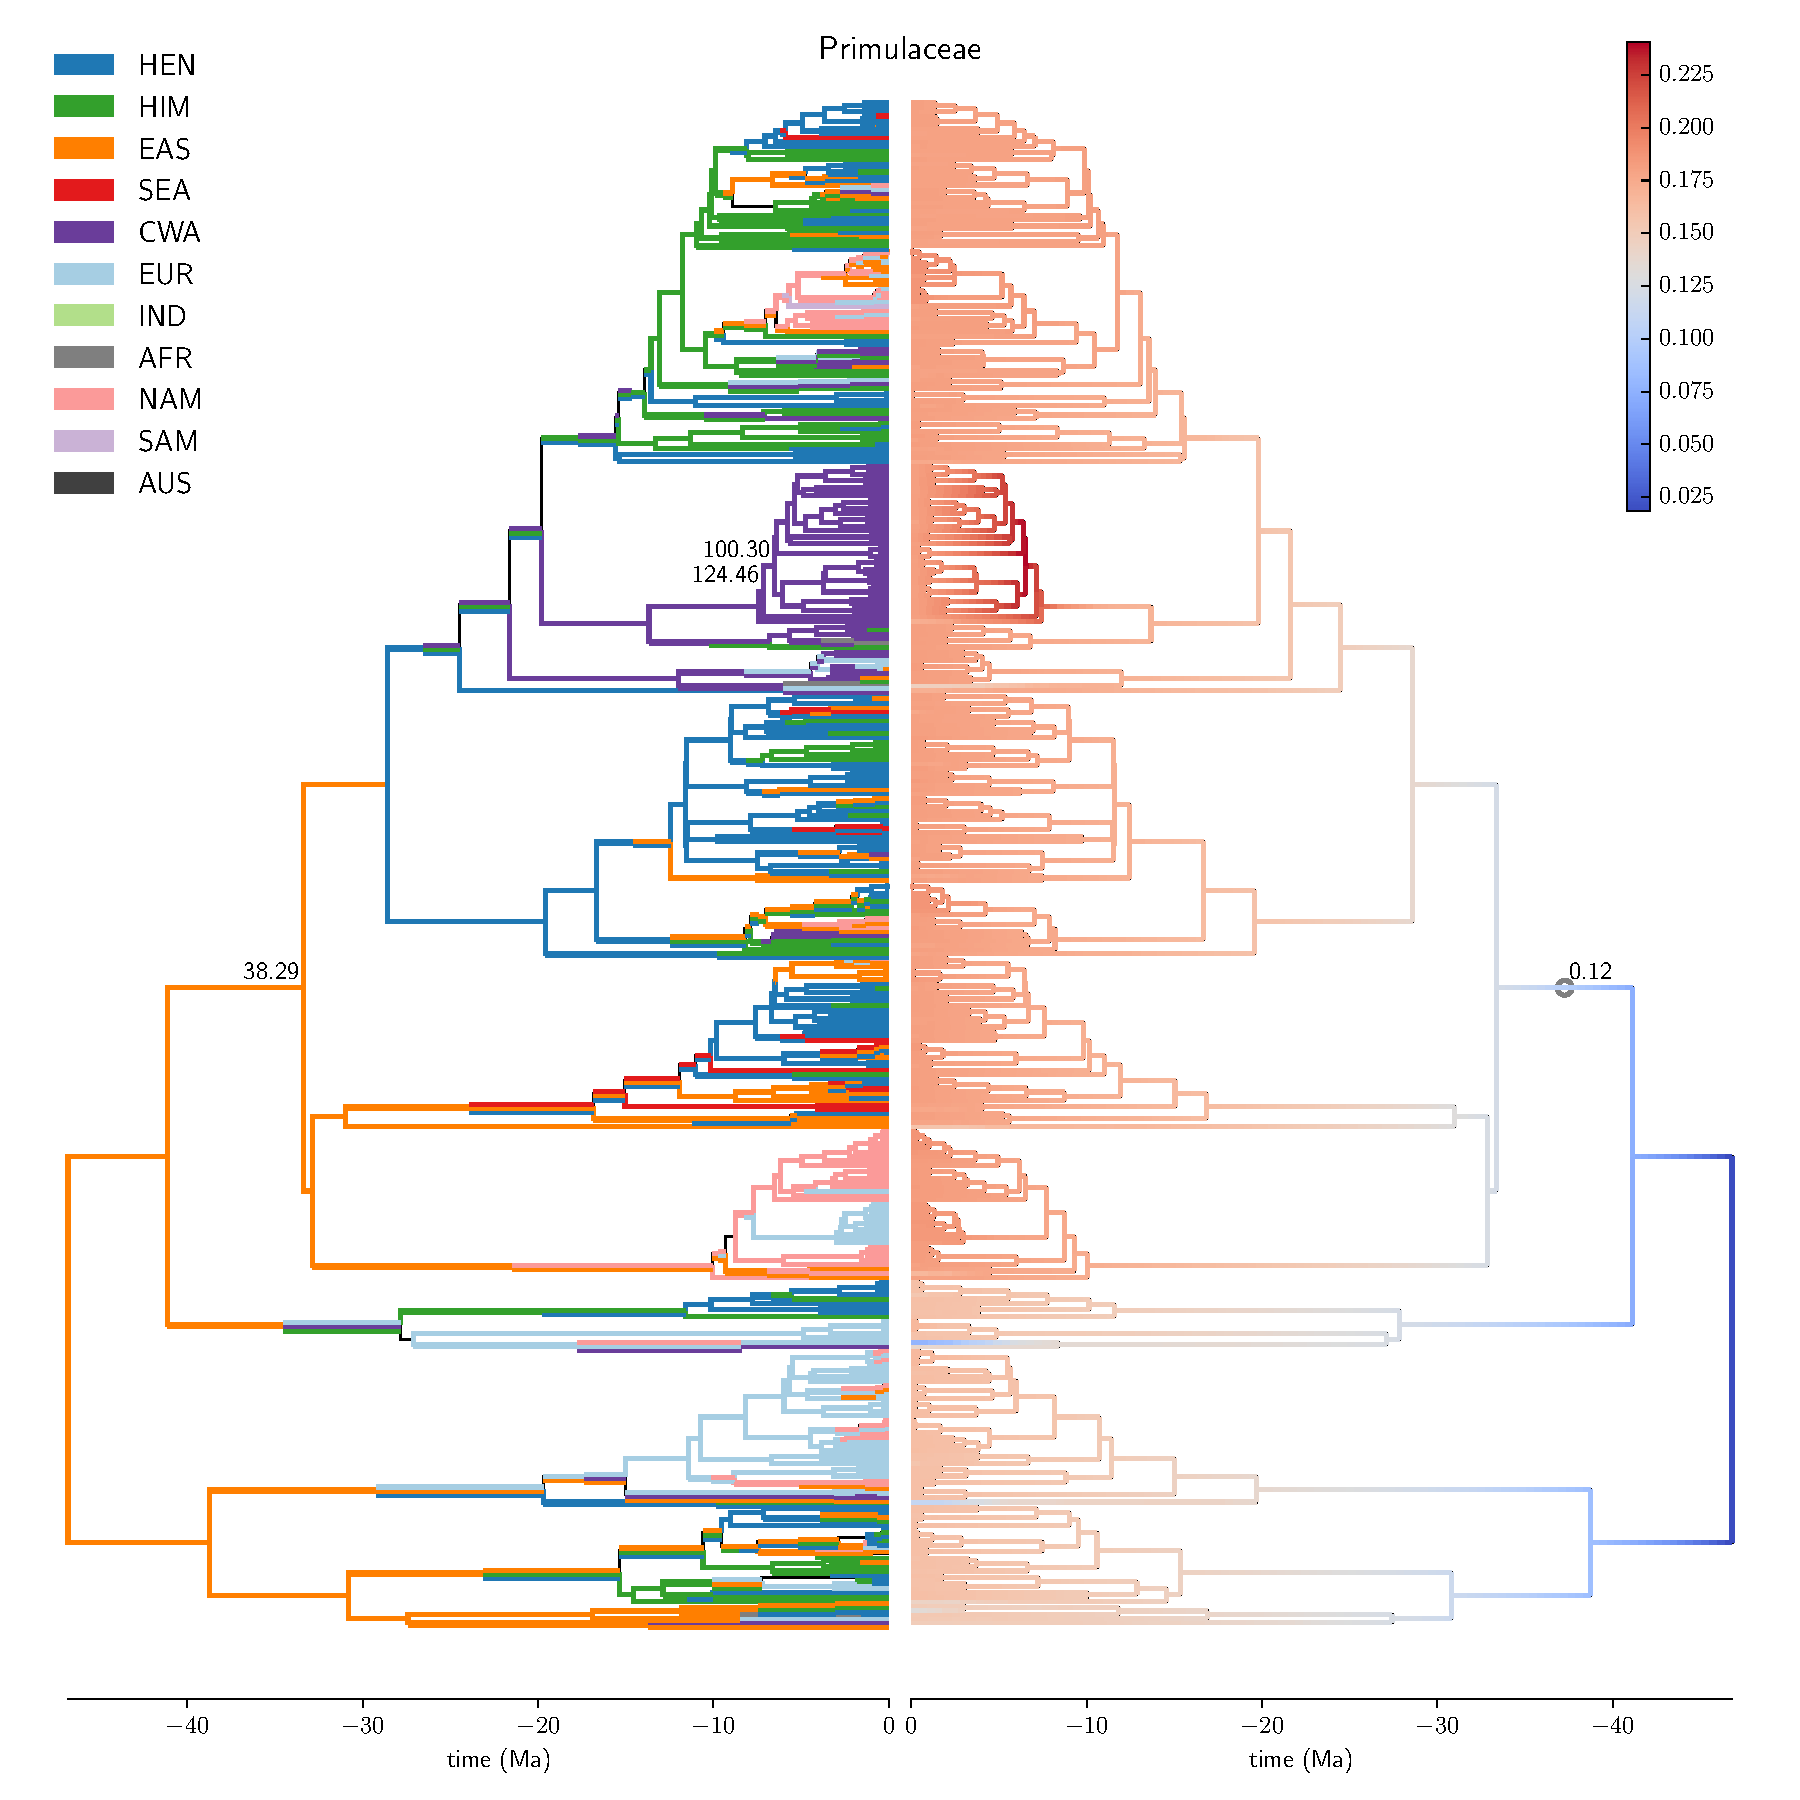
\includegraphics[width=.99\linewidth]{figures/Primulaceae-supfig.pdf}
\label{fig:allium}
\caption{Primulaceae}
\end{subfigure}
\end{figure}

\begin{figure}
  \ContinuedFloat
\begin{subfigure}{\textwidth}
\centering
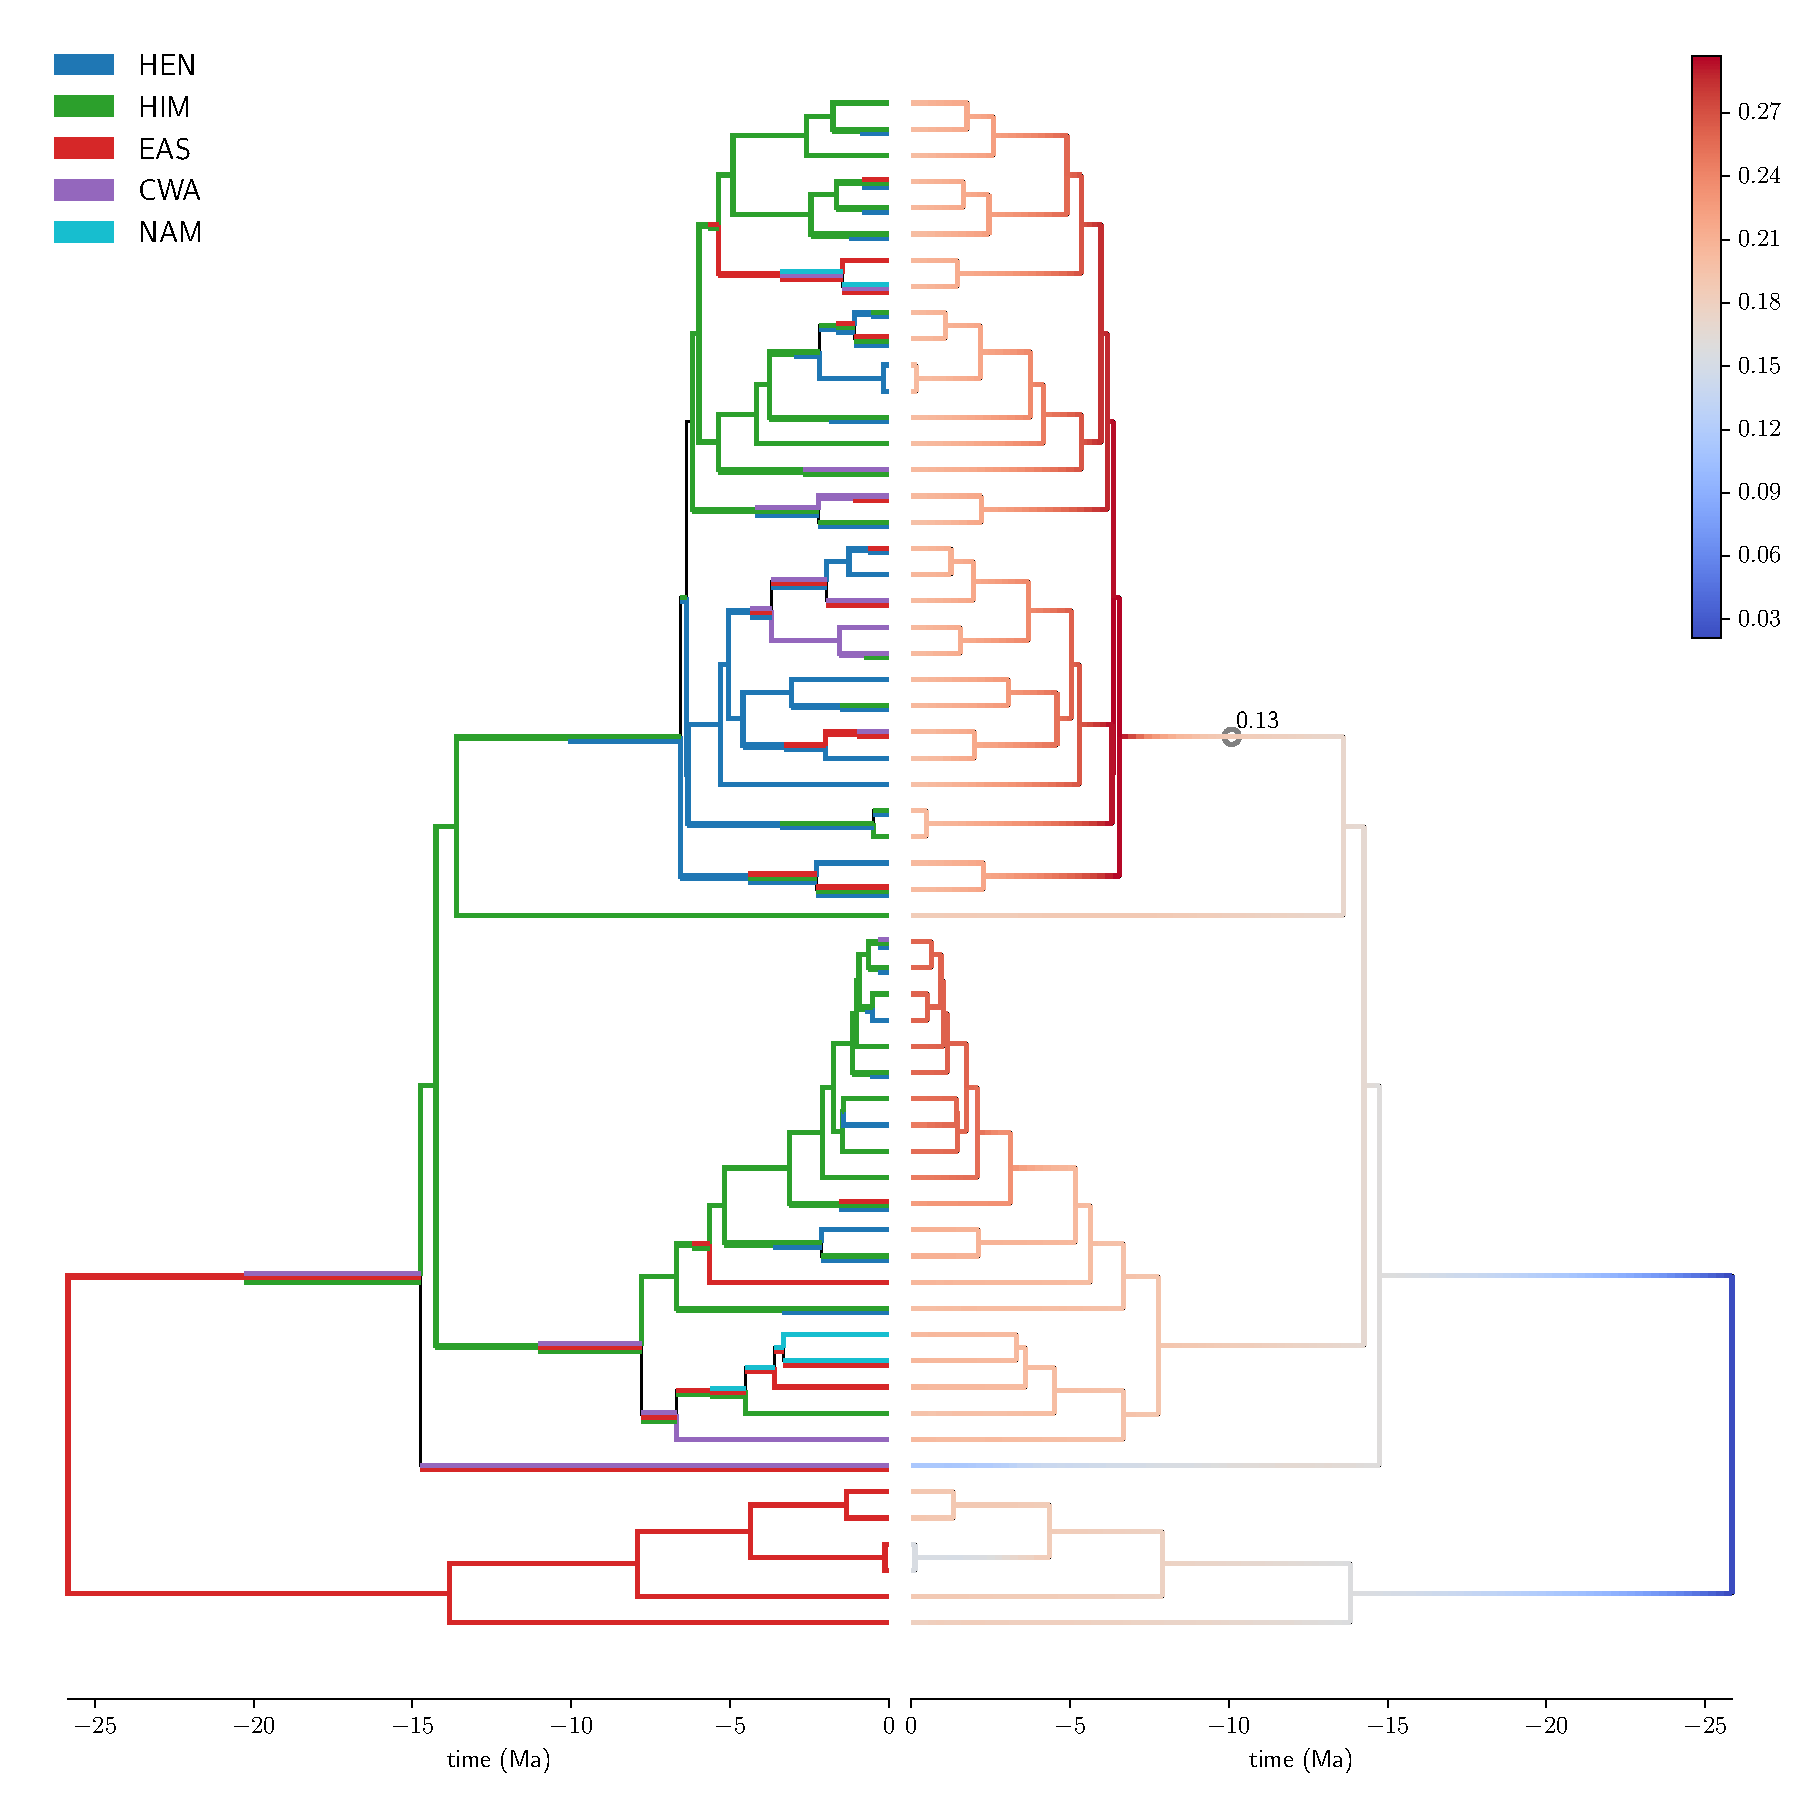
\includegraphics[width=.99\linewidth]{figures/Rhodiola-supfig.pdf}
\label{fig:allium}
\caption{\textit{Rhodiola}}
\end{subfigure}
\end{figure}

\begin{figure}
  \ContinuedFloat
\begin{subfigure}{\textwidth}
\centering
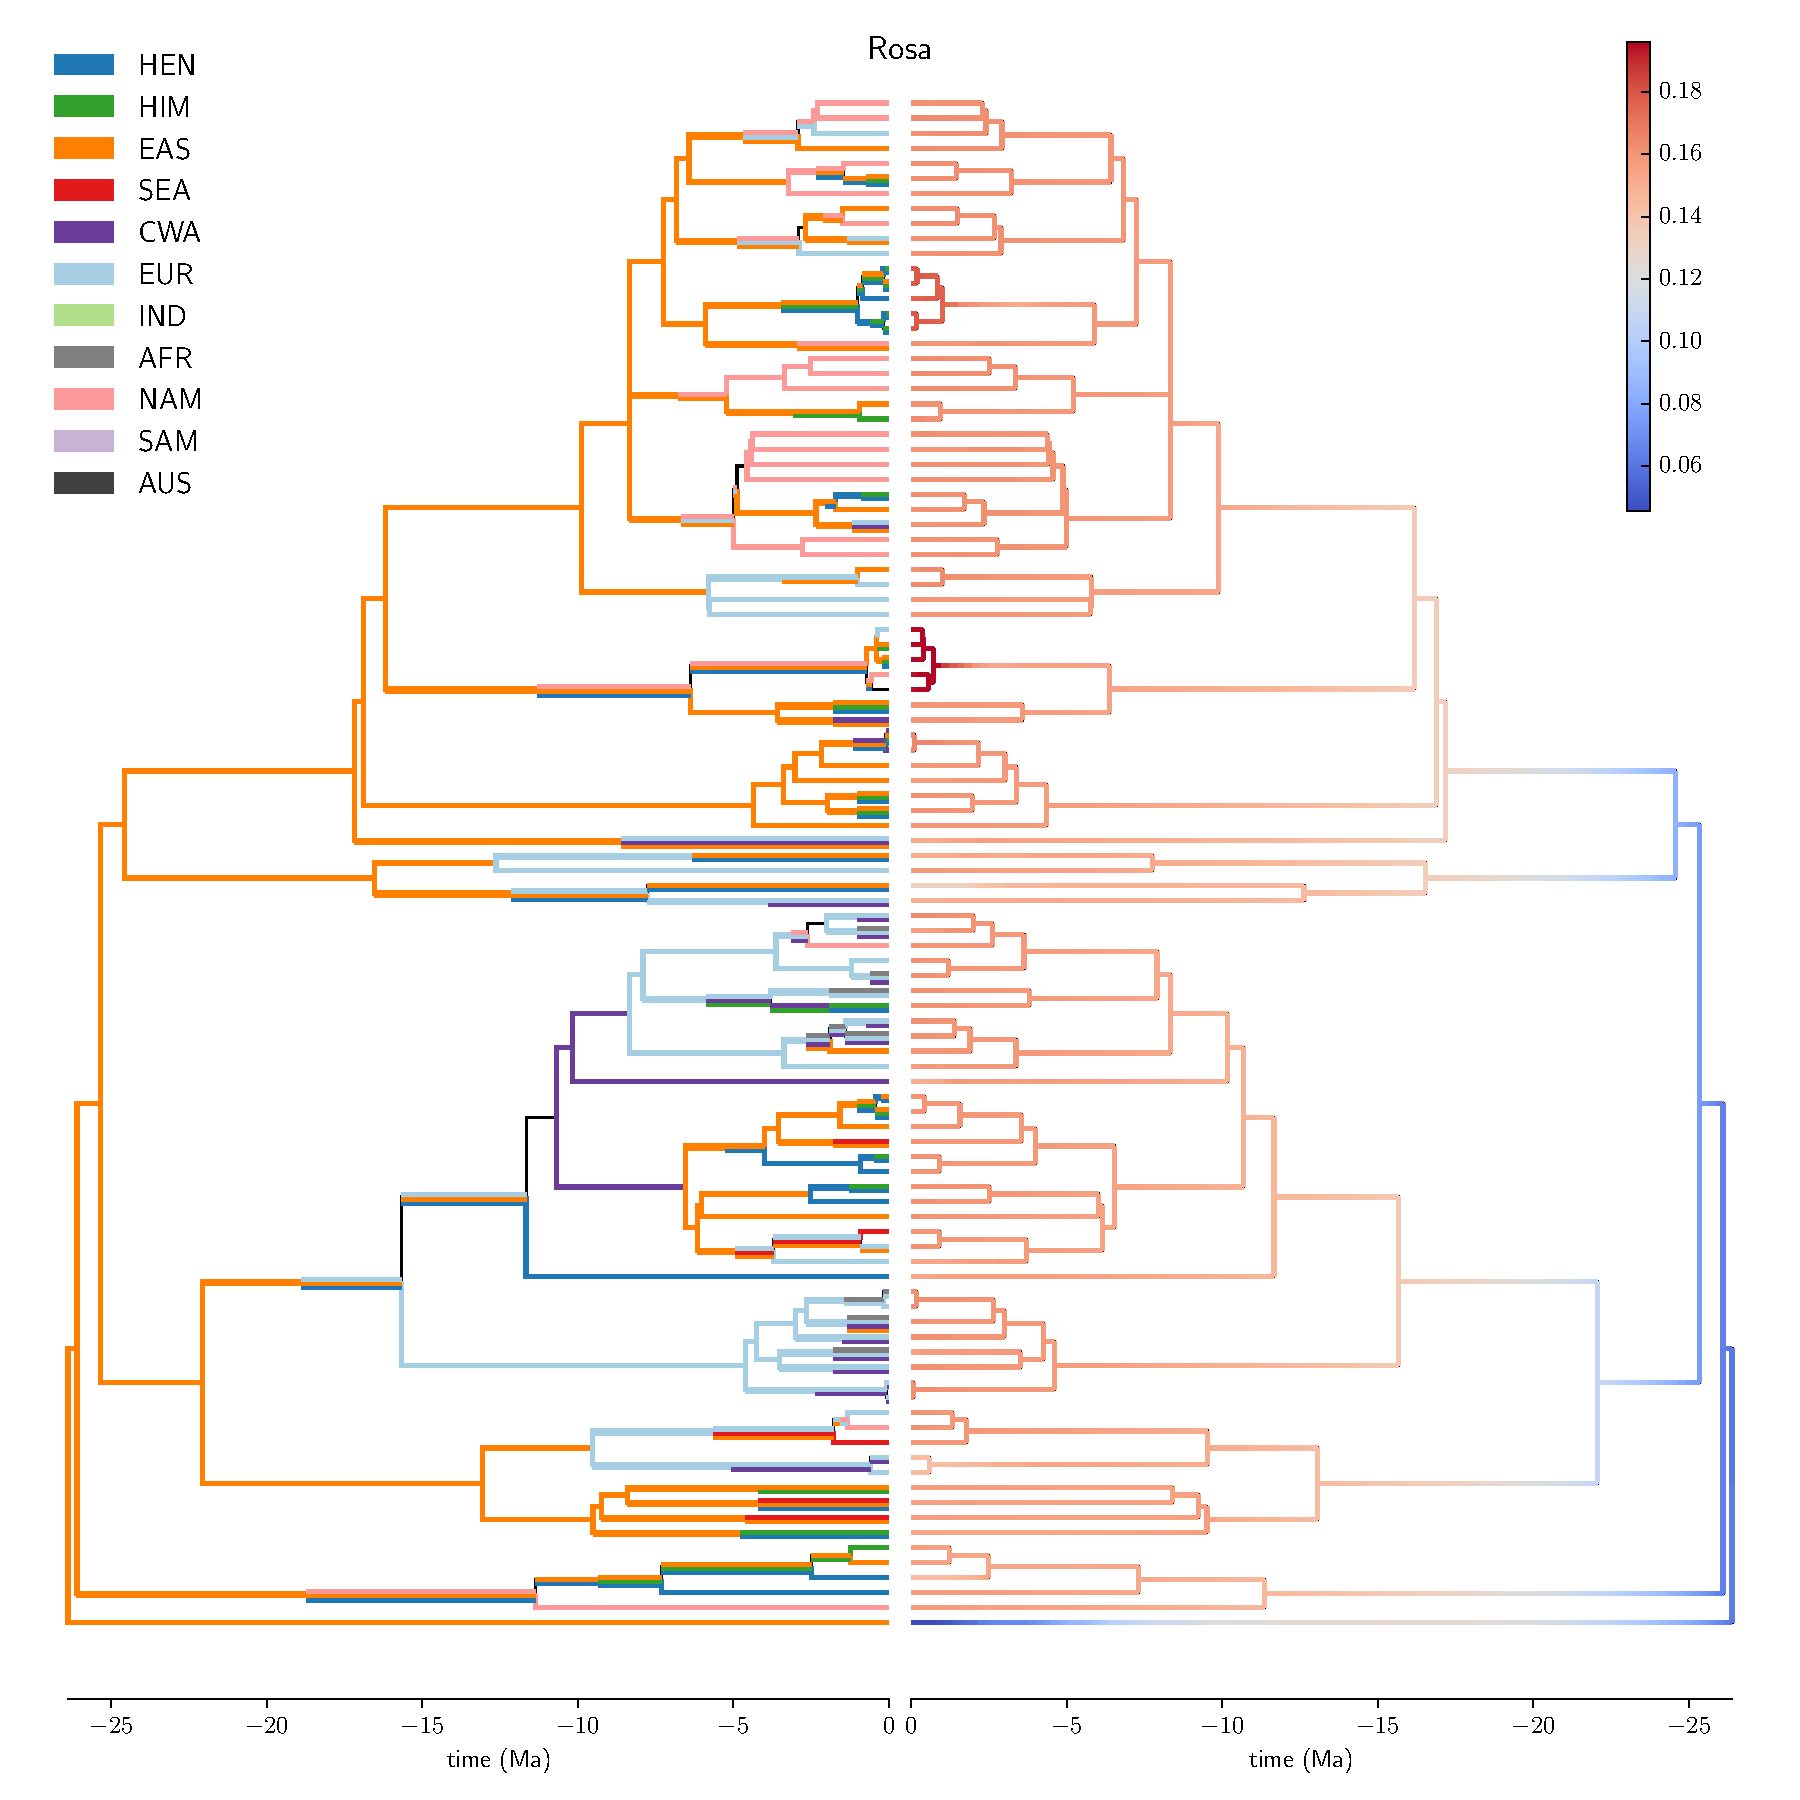
\includegraphics[width=.99\linewidth]{figures/Rosa-supfig.pdf}
\label{fig:allium}
\caption{\textit{Rosa}}
\end{subfigure}
\end{figure}

\begin{figure}
  \ContinuedFloat
\begin{subfigure}{\textwidth}
\centering
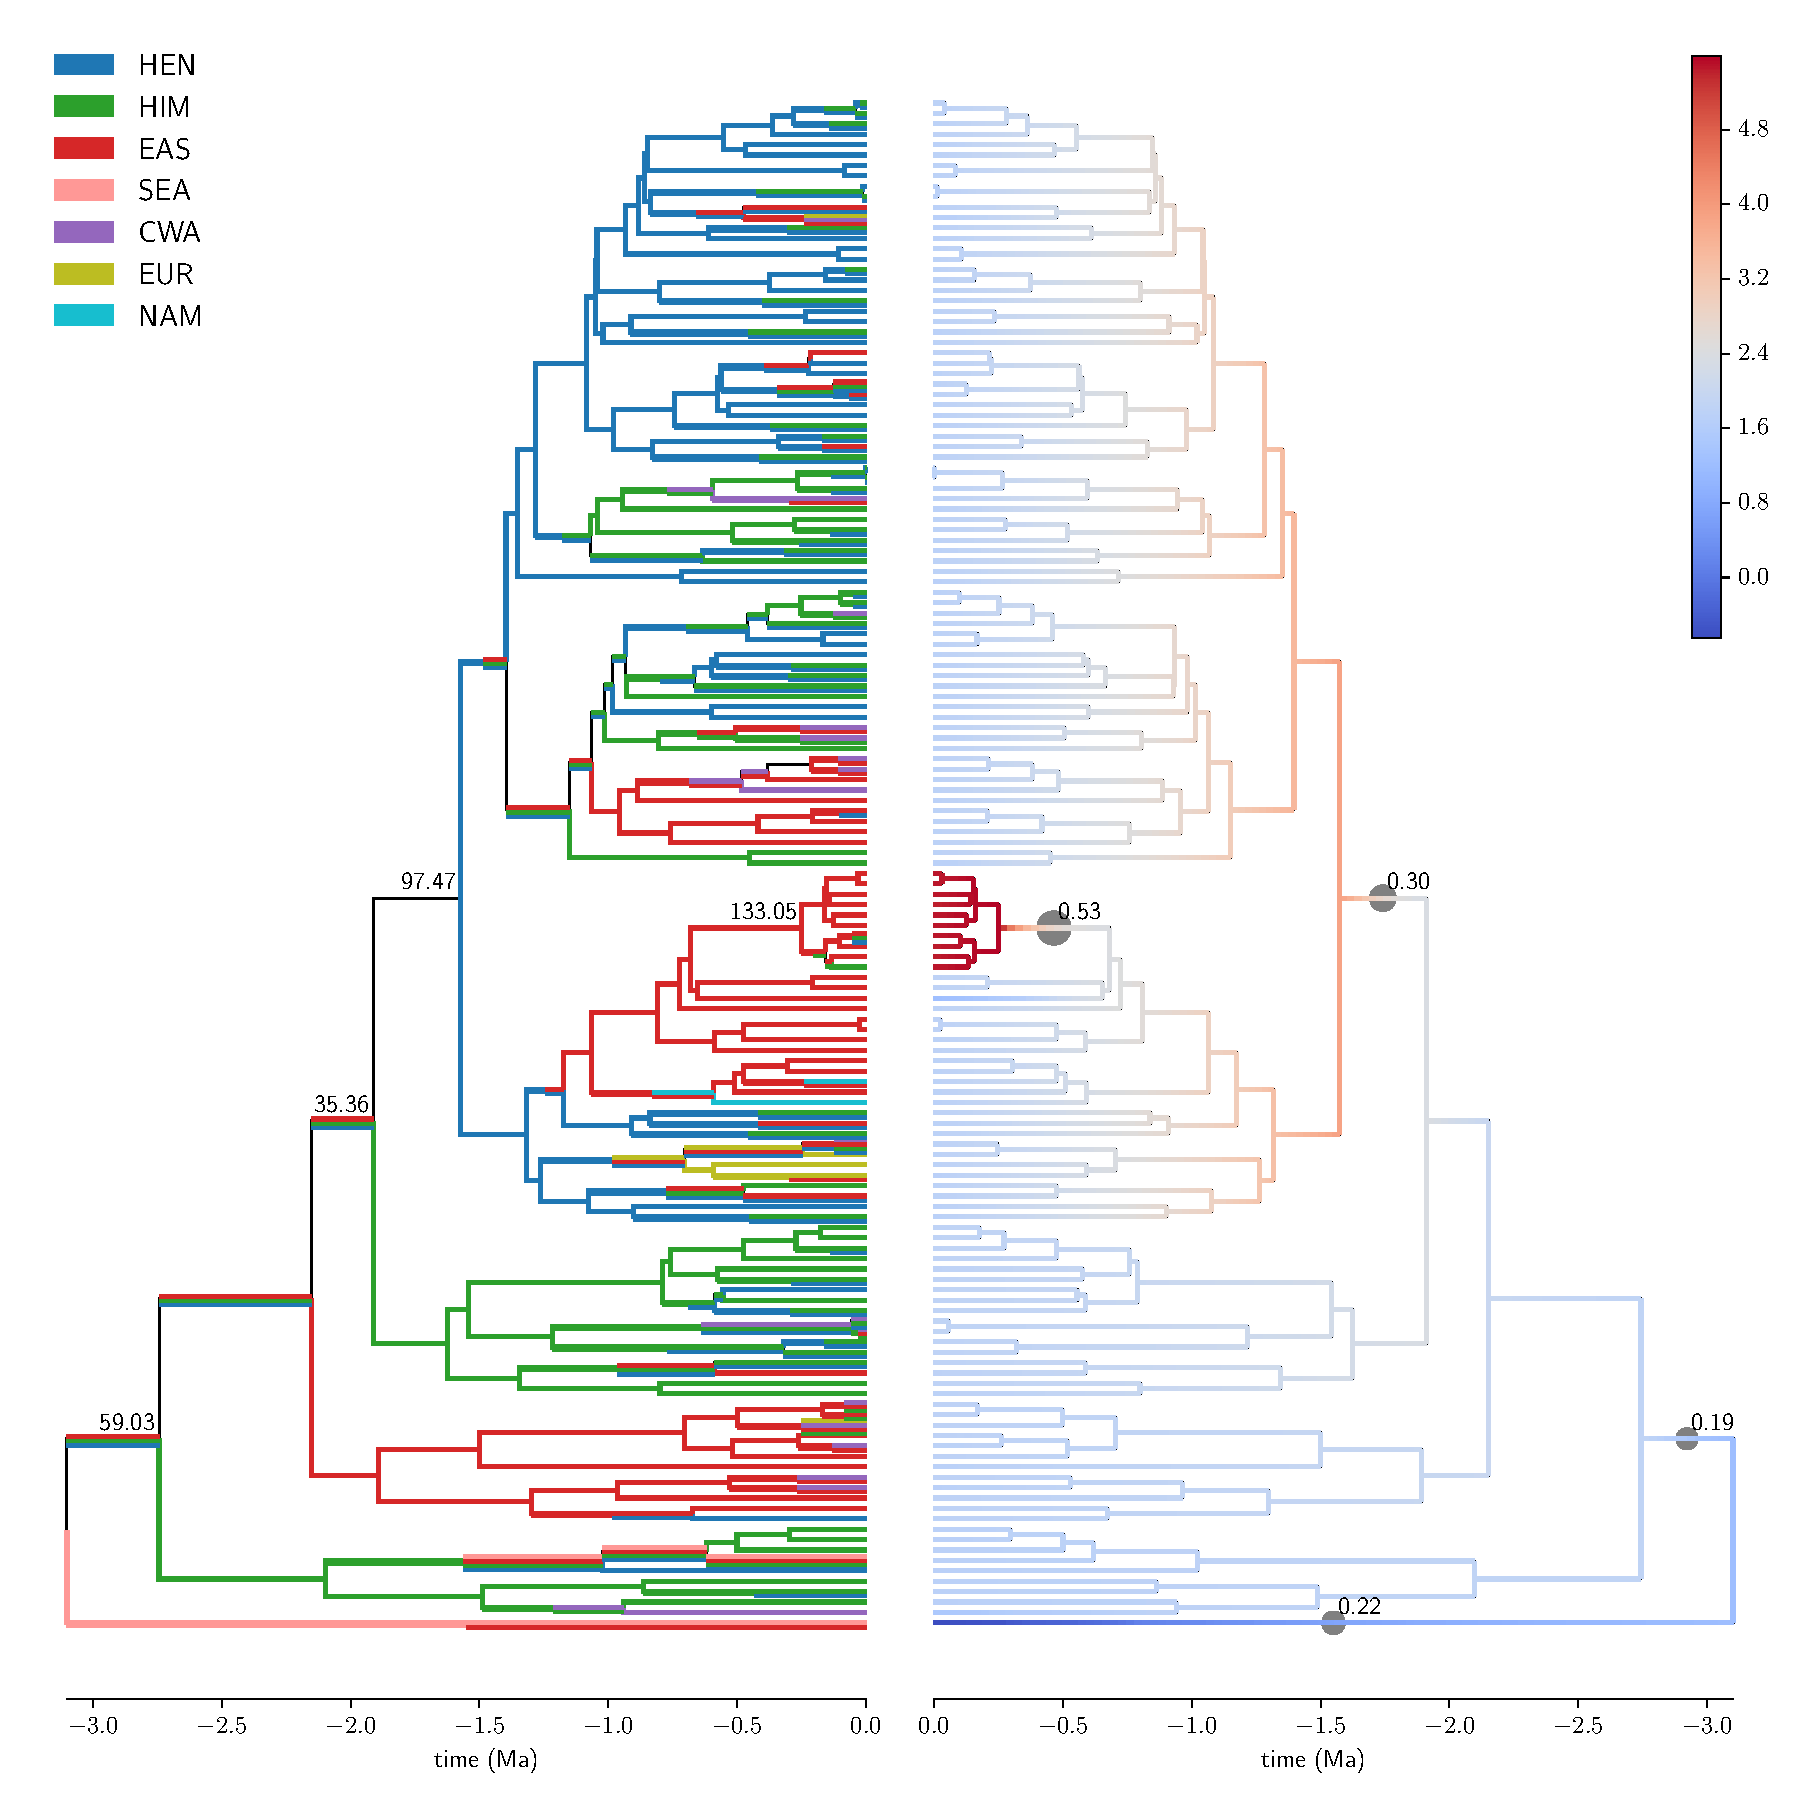
\includegraphics[width=.99\linewidth]{figures/Saussurea-supfig.pdf}
\label{fig:allium}
\caption{\textit{Saussurea}}
\end{subfigure}
\end{figure}

\begin{figure}
  \ContinuedFloat
\begin{subfigure}{\textwidth}
\centering
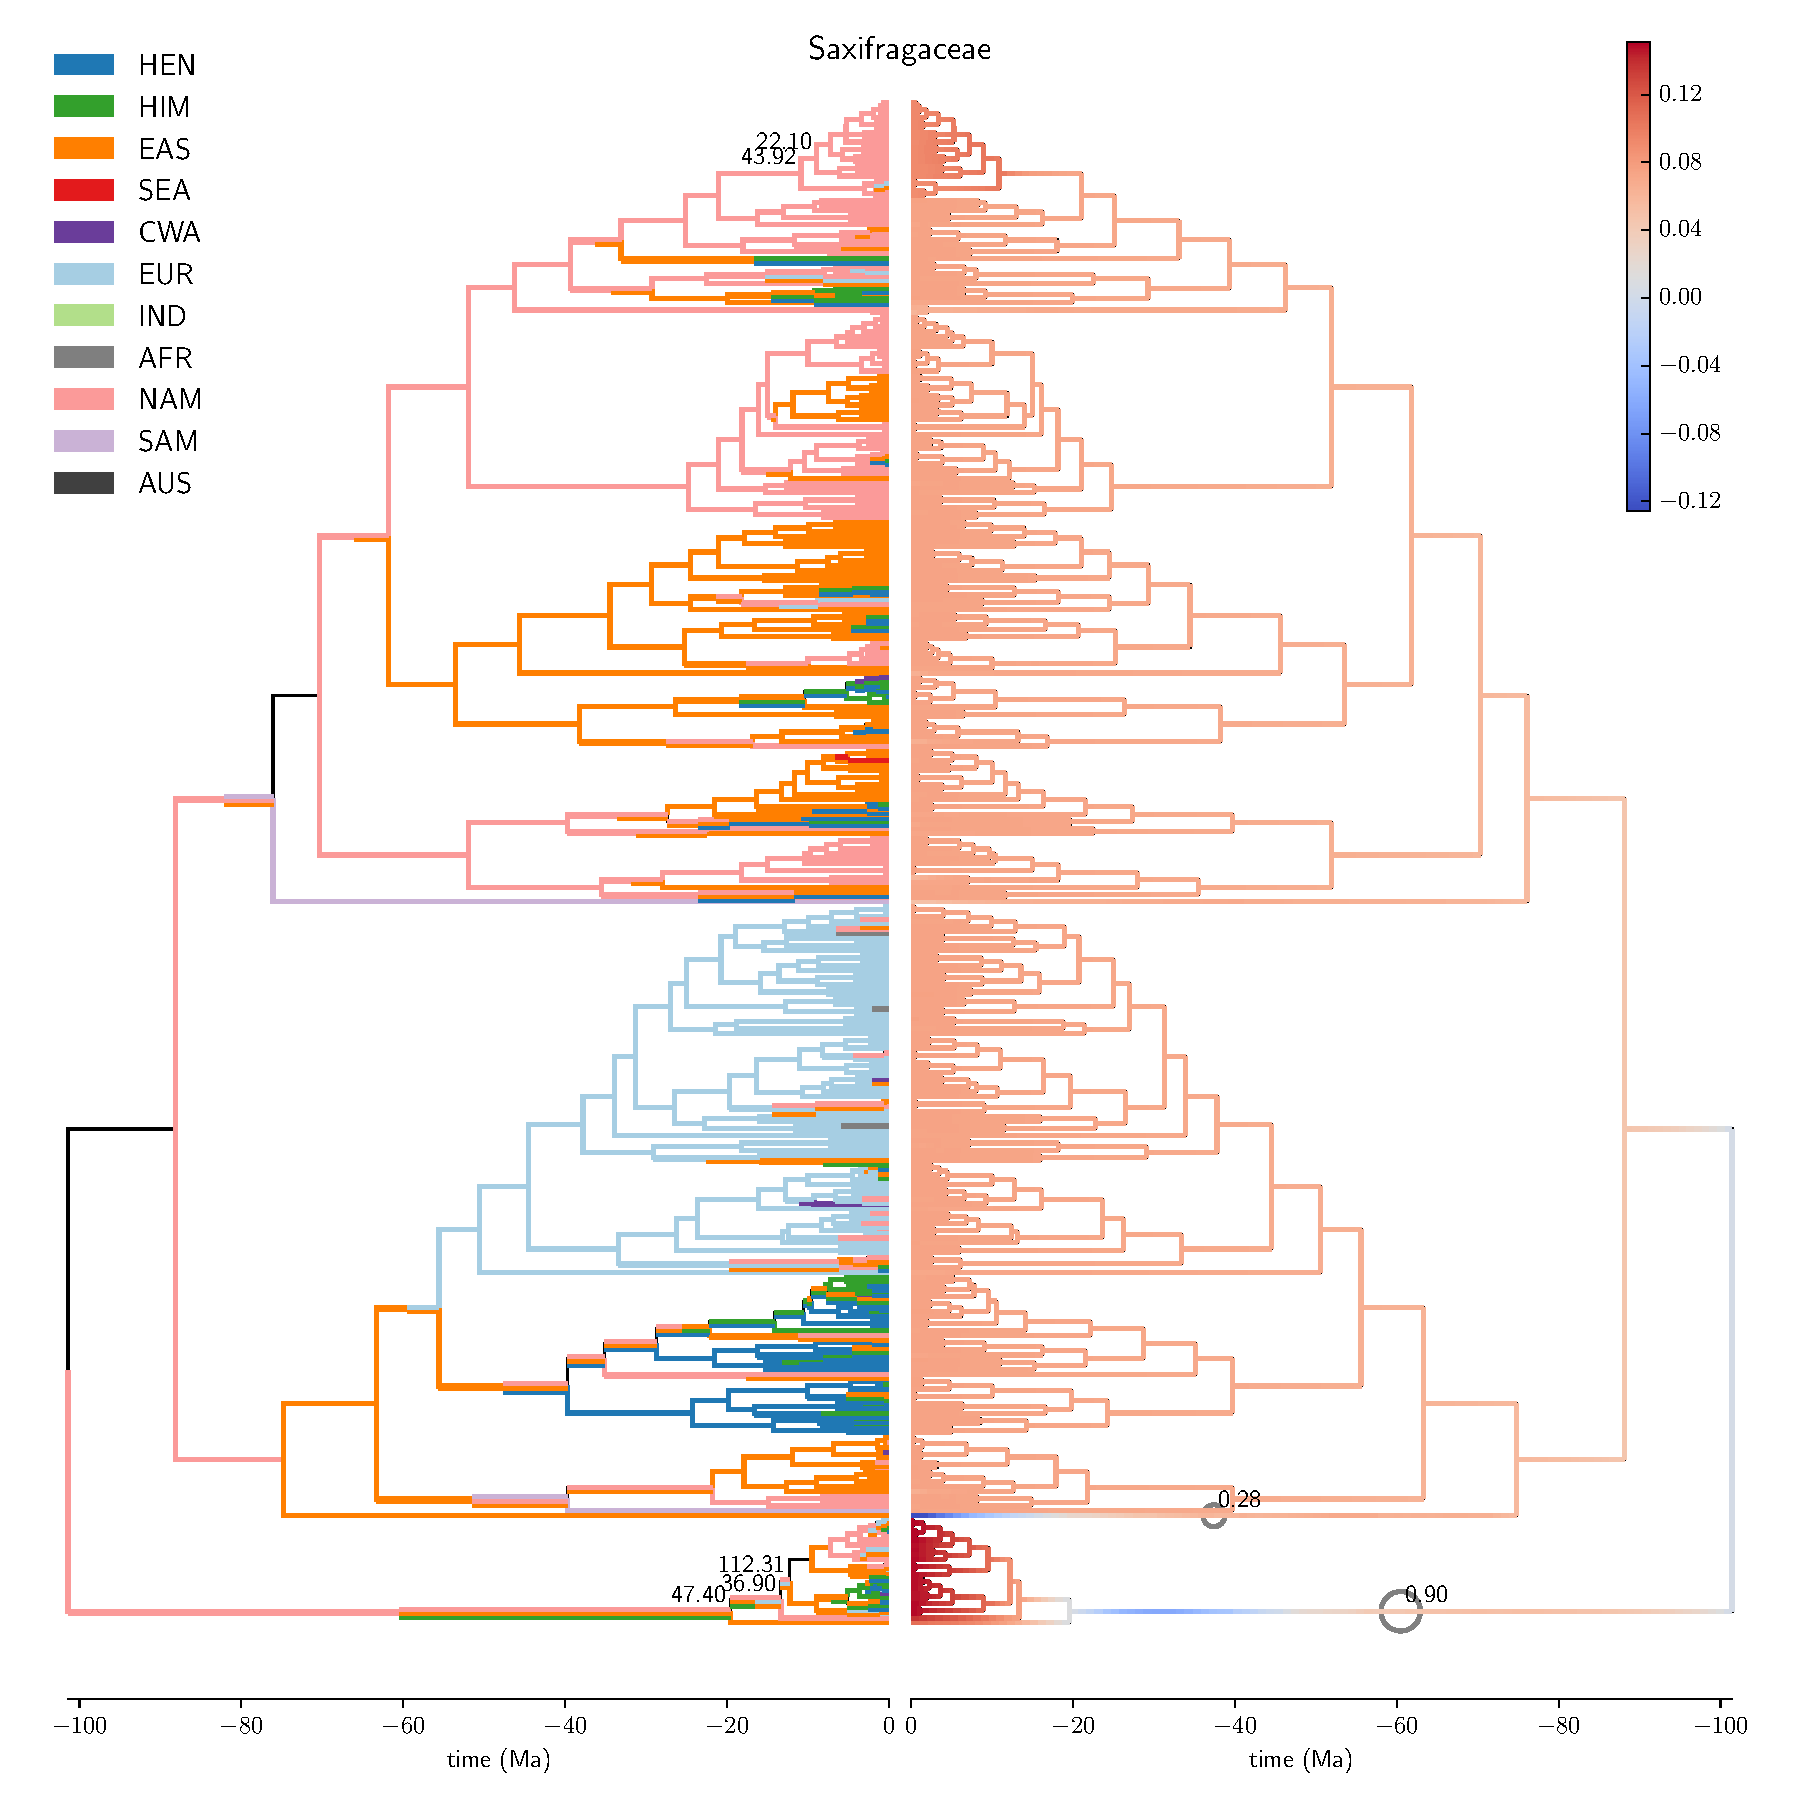
\includegraphics[width=.99\linewidth]{figures/Saxifragaceae-supfig.pdf}
\label{fig:allium}
\caption{Saxifragaceae-Grossulariaceae}
\end{subfigure}
\end{figure}

\begin{figure}
  \ContinuedFloat
\begin{subfigure}{\textwidth}
\centering
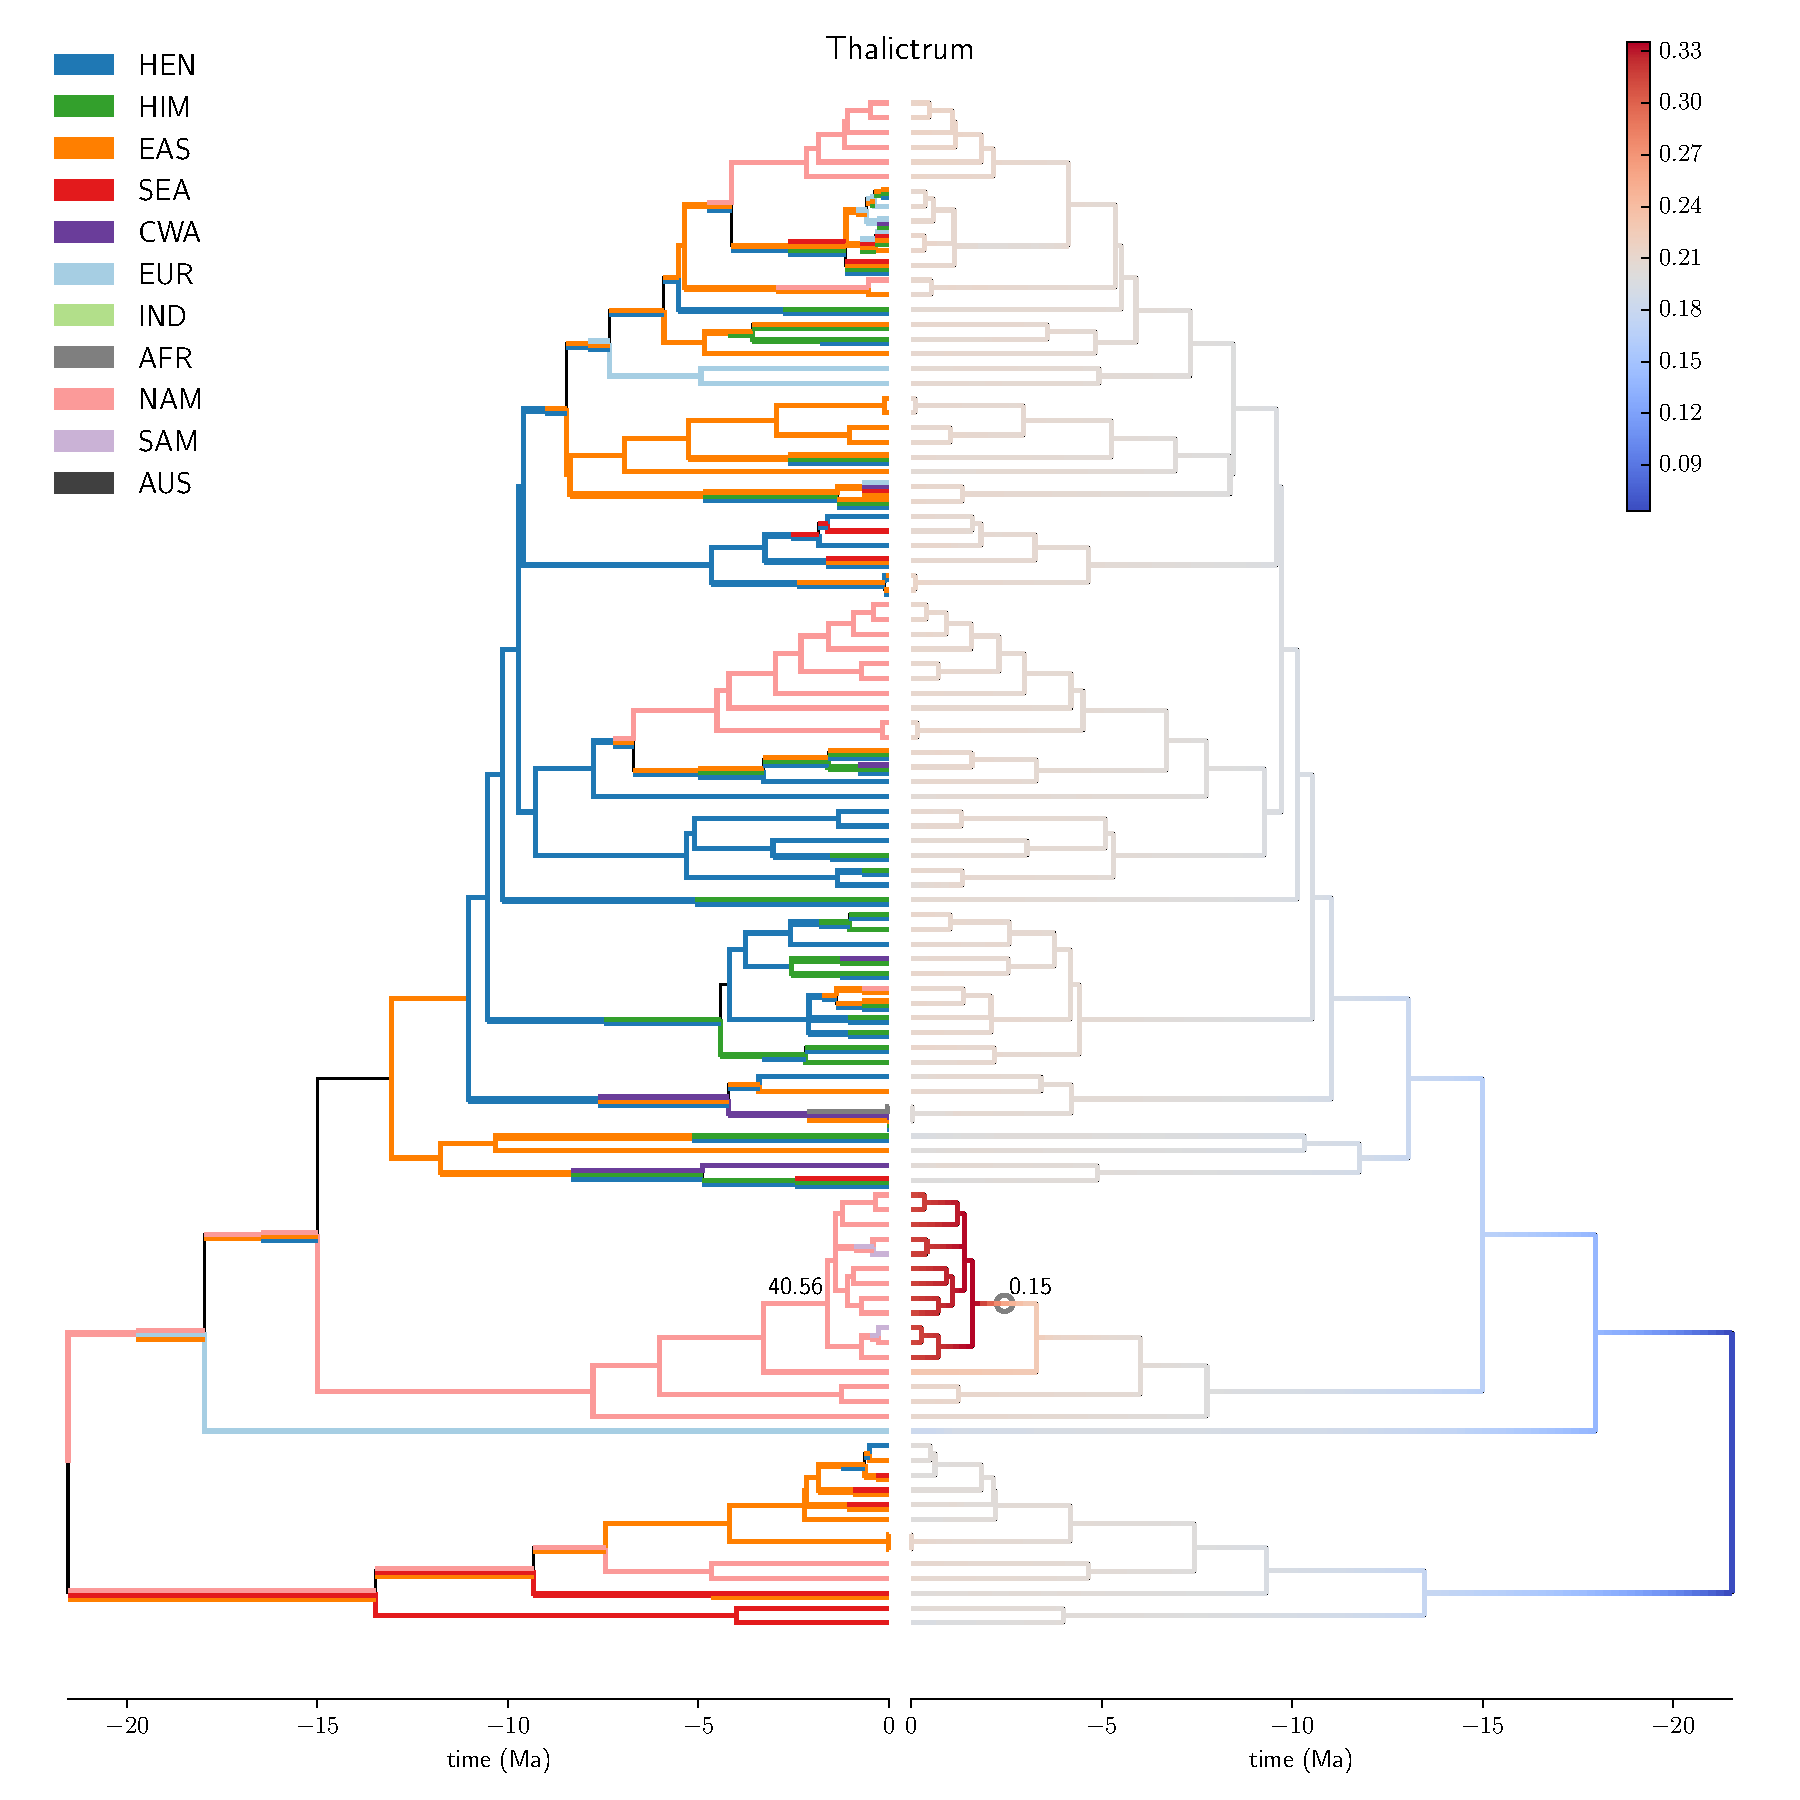
\includegraphics[width=.99\linewidth]{figures/Thalictrum-supfig.pdf}
\label{fig:allium}
\caption{\textit{Thalictrum}}
\end{subfigure}
\end{figure}

\begin{figure}
\centering
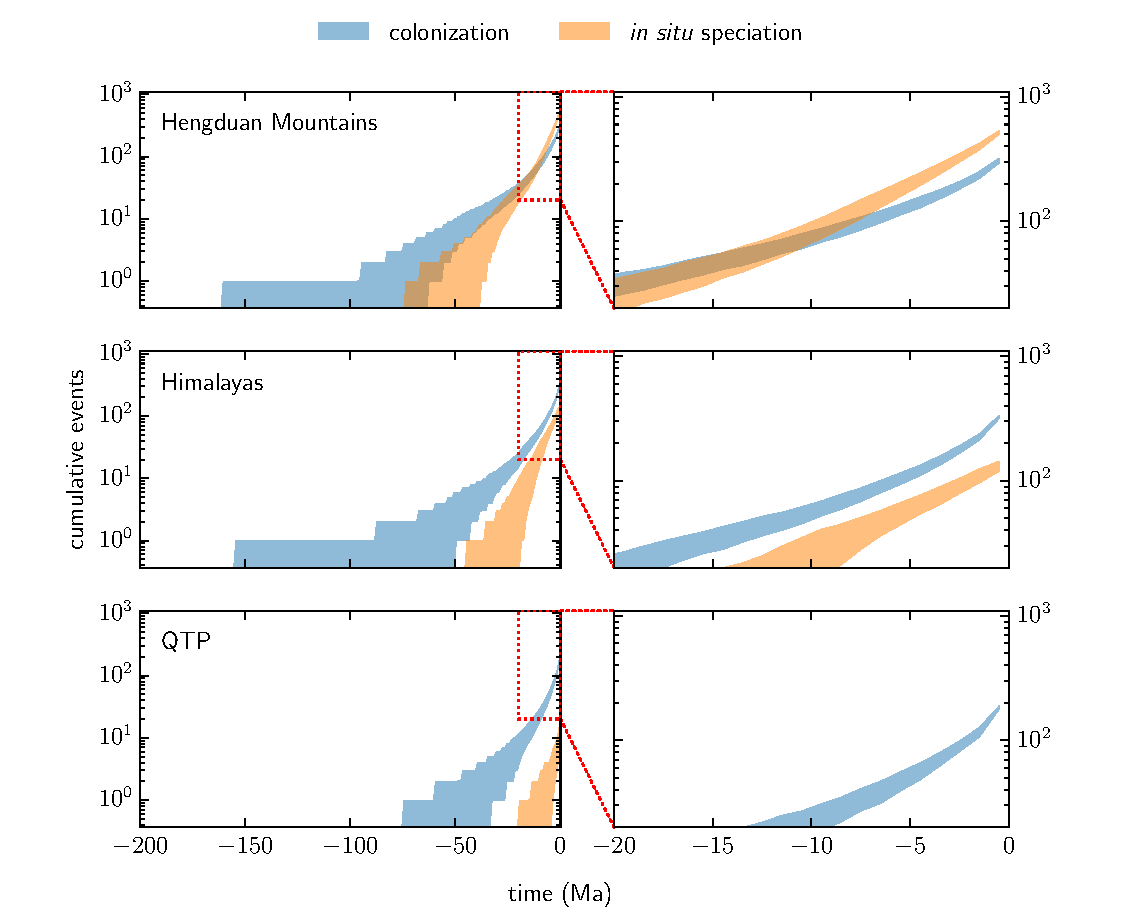
\includegraphics[width=.99\linewidth]{figures/cumulative-events-qtp.pdf}
\caption{Cumulative numbers of colonization and \textit{in situ}
  speciation events in 19 plant clades through time, as described in
  Figure 2. Here, the same analysis is shown, except that is based on
  ancestral range reconstructions in which the Himlayas and QTP were
  coded as distinct areas. The dynamics of the Hengduan region are
  essentially unchanged from the original analysis.}
\label{fig:cumevents:qtp}
\end{figure}

\begin{figure}
\centering
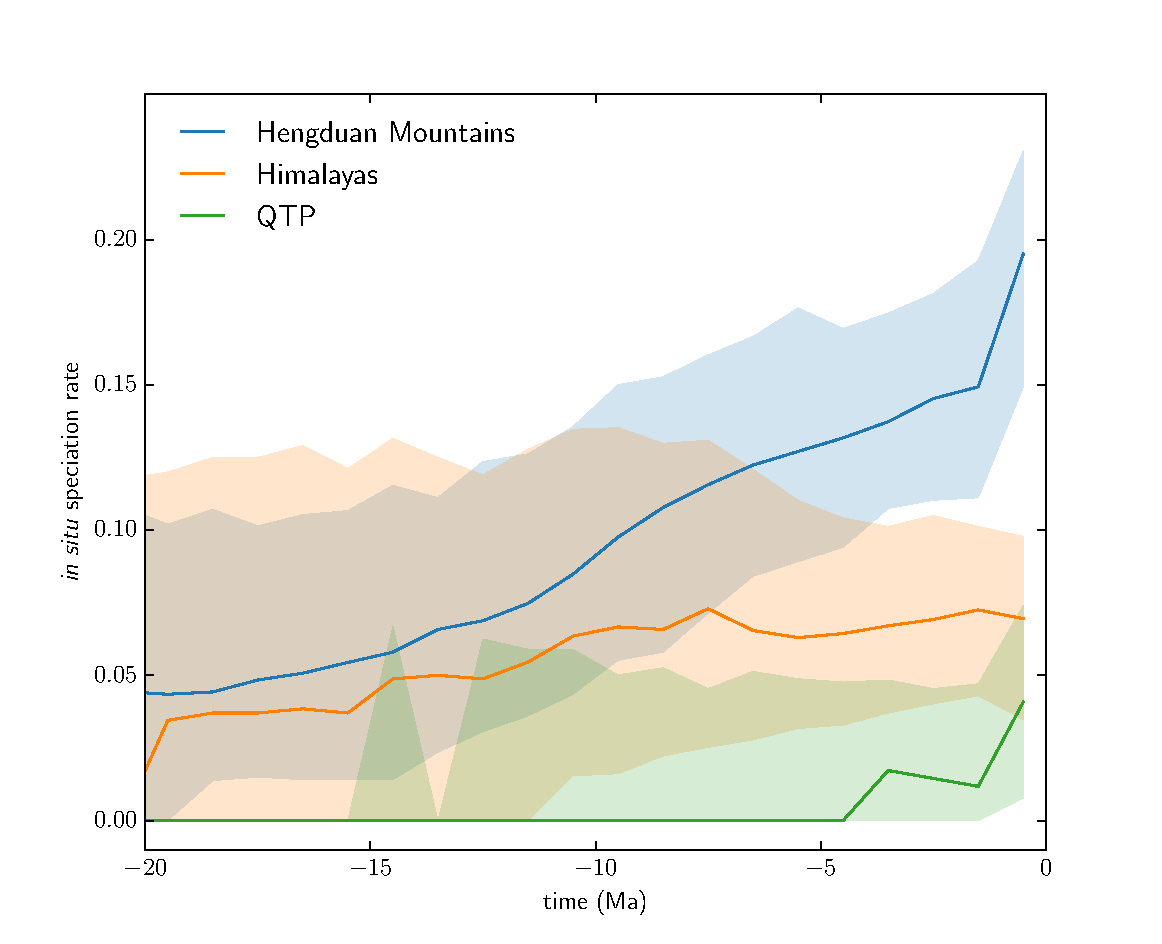
\includegraphics[width=.99\linewidth]{figures/speciation-rates-qtp.pdf}
\caption{Rolling estimates of \textit{in situ} speciation rates
  through time, as described in Figure 3, showing the results from
  treating the Himalayas and QTP as distinct areas. The dynamics of
  the Hengduan region are essentially unchanged from the original
  analysis.}
\label{fig:speciation:qtp}
\end{figure}

\begin{figure}
\centering
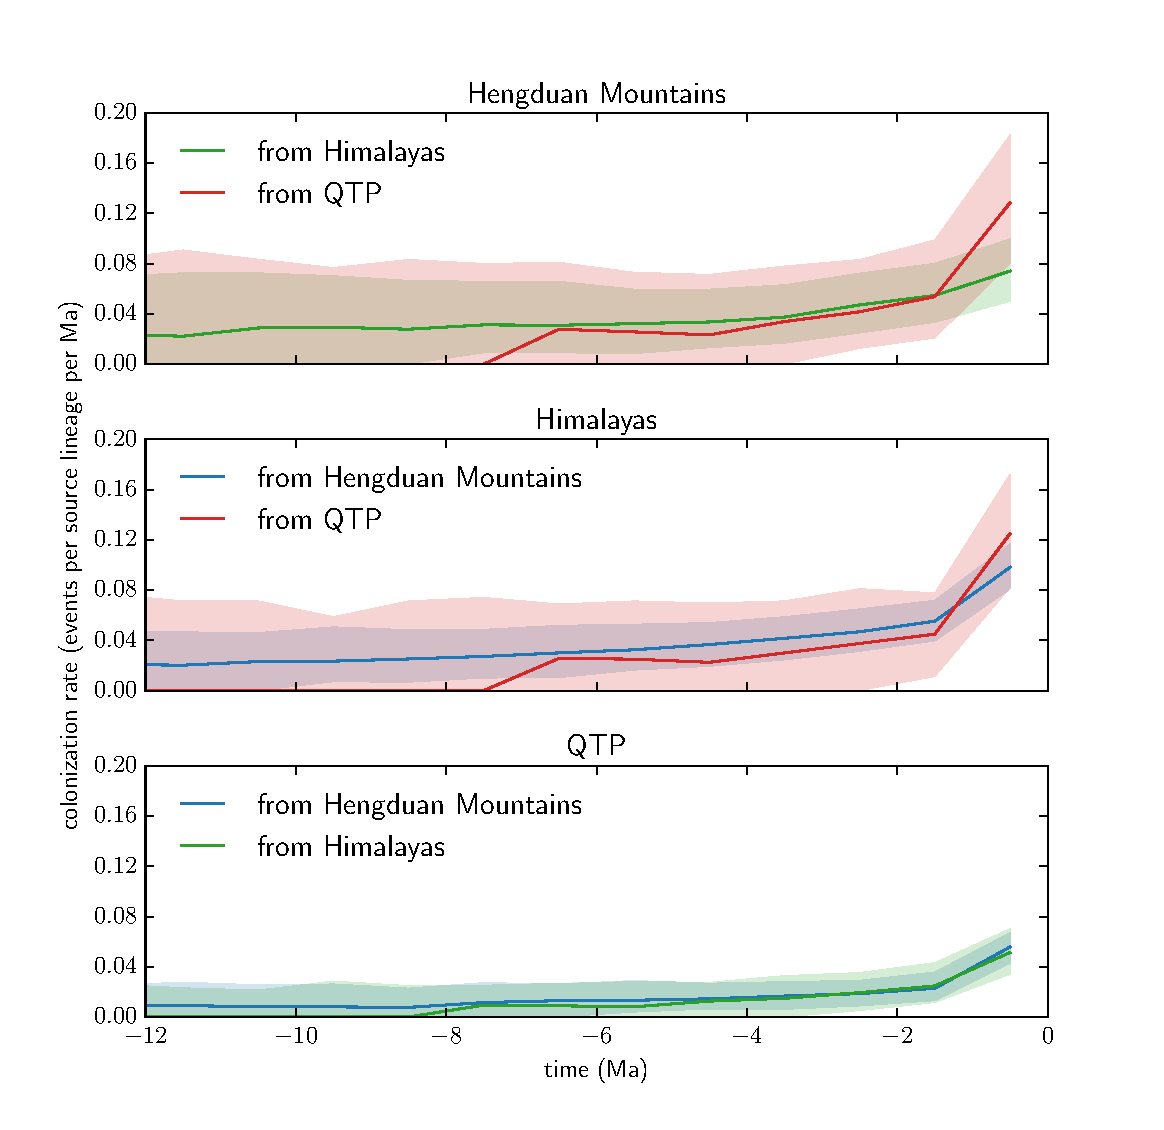
\includegraphics[width=.99\linewidth]{figures/dispersal-rates-qtp.pdf}
\caption{Rolling estimates of colonization rates through time, as
  described in Figure 4, showing the results from treating the
  Himalayas and QTP as distinct areas. The dynamics of the Hengduan
  region are essentially unchanged from the original analysis.}
\label{fig:dispersal:qtp}
\end{figure}

\begin{figure}
\centering
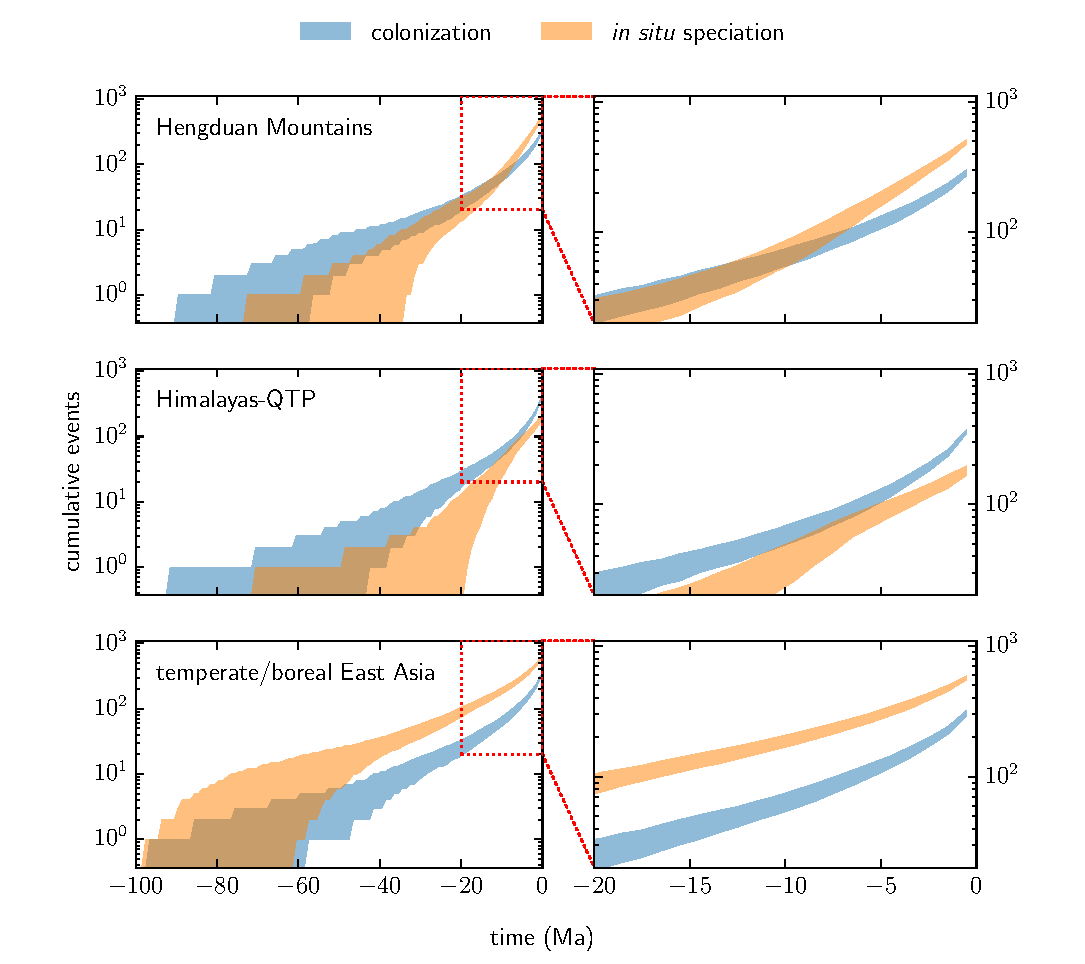
\includegraphics[width=.99\linewidth]{figures/cumulative-events-angiosperms.pdf}
\caption{Cumulative numbers of colonization and \textit{in situ}
  speciation events in 19 plant clades through time, as described in
  Figure 2. Here, the same analysis is shown, except that is based
  only on the 17 angiosperm clades. The dynamics of the Hengduan
  region are essentially unchanged from the original analysis.}
\label{fig:cumevents:angios}
\end{figure}

\begin{figure}
\centering
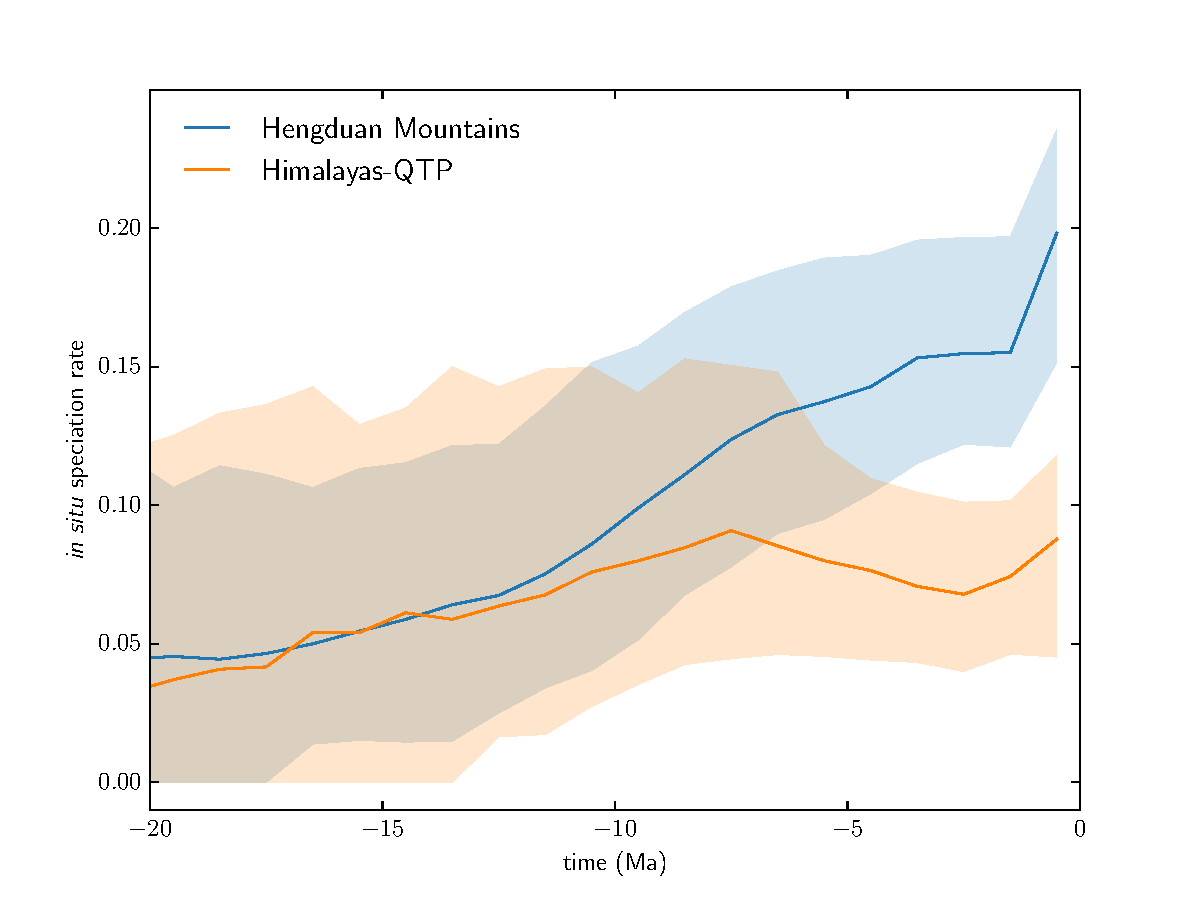
\includegraphics[width=.99\linewidth]{figures/speciation-rates-angiosperms.pdf}
\caption{Rolling estimates of \textit{in situ} speciation rates
  through time, as described in Figure 3. Here, the same analysis is
  shown, except that is based only on the 17 angiosperm clades. The
  dynamics of the Hengduan region are essentially unchanged from the
  original analysis.}
\label{fig:speciation:angios}
\end{figure}

\begin{figure}
\centering
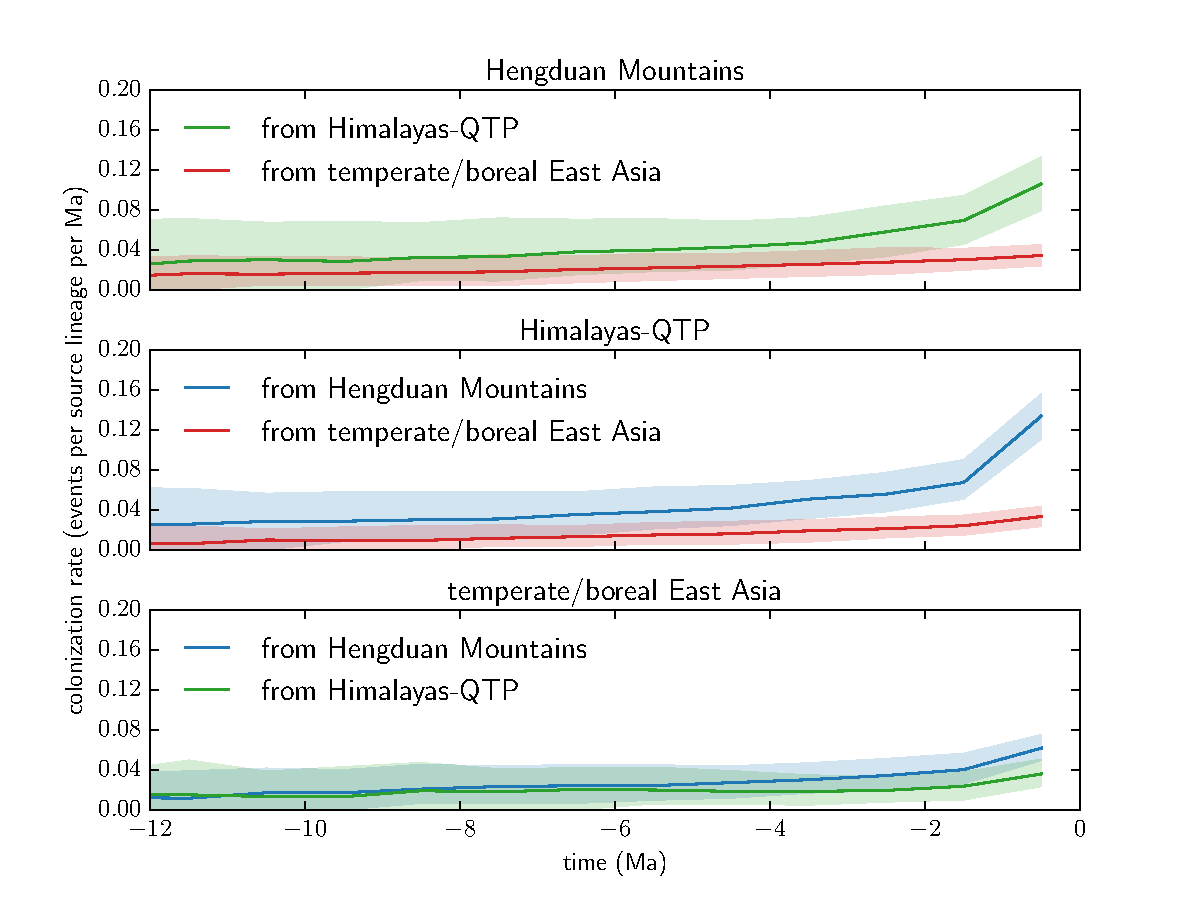
\includegraphics[width=.99\linewidth]{figures/dispersal-rates-angiosperms.pdf}
\caption{Rolling estimates of colonization rates through time, as
  described in Figure 4. Here, the same analysis is shown, except that
  is based only on the 17 angiosperm clades. The dynamics of the
  Hengduan region are essentially unchanged from the original
  analysis.}
\label{fig:dispersal:angios}
\end{figure}

%%% Local Variables:
%%% mode: latex
%%% TeX-master: "SI"
%%% End:
